\subsection[\englishfont 2.3 面向车载信息物理融合的质量-开销均衡优化]{2.3 面向车载信息物理融合的质量-开销均衡优化}

\begin{frame}{研究贡献}
\newBackground
\begin{center}
\begin{textblock*}{\textwidth}(-2cm,1.8cm)
  \small \englishfont \colorbox{cqublue}{\color{white}{创新的服务质量与系统开销均衡策略是实现}}
\end{textblock*}
\end{center}

\begin{center}
\begin{textblock*}{\textwidth}(-2cm,2.3cm)
  \small \englishfont \colorbox{cqublue}{\color{white}{{\color{yellow}{高质量、低成本和可扩展}}\hspace{0.25em}VCPS的{\color{yellow}{理论保障}}}}
\end{textblock*}
\end{center}

\begin{center}
\begin{textblock*}{\textwidth}(-2.1cm,3.2cm)
\begin{minipage}[t]{0.6\textwidth}
\begin{itemize}[itemsep=0.2\baselineskip] \englishfont 
	\item[\ding{111}] {{\color{cqublue}{\textbf{问题}}}:{\color{red}{双目标优化}}问题}
	\begin{itemize}[itemsep=0.2\baselineskip]
	\begin{small}
		\item[\ding{226}] \underline{最大化}VCPS质量:视图及时性和一致性
		\item[\ding{226}] \underline{最小化}VCPS开销:信息冗余度、感知开销和传输开销
	\end{small}
	\end{itemize}
	\item[\ding{111}] {{\color{cqublue}{\textbf{算法}}}:基于多目标的多智能体深度强化学习算法 ({\color{red}{MAMO}})} 
	\item[\ding{111}] {{\color{cqublue}{\textbf{实验}}}:有效实现质量和开销的均衡} 
\end{itemize}
\end{minipage}
\end{textblock*}
\end{center}


\begin{center}
\begin{textblock*}{\textwidth}(-1.6cm,7.5cm)
\fbox{\begin{minipage}[t]{0.7\textwidth}\englishfont \tiny [5] LIU K,\underline{\textcolor{cqublue}{XU X}}, DAI P, et al. \textcolor{cqublue}{Cooperative sensing and uploading for quality-cost tradeoff of digital twins in VEC}[J]. IEEE Transactions on Consumer Electronics (\textcolor{red}{TCE}), under minor revision. (中科院SCI 2区)
\end{minipage}}
\end{textblock*}
\end{center}

\begin{center}
\begin{textblock*}{\textwidth}(6.2cm,2cm)
\begin{figure}
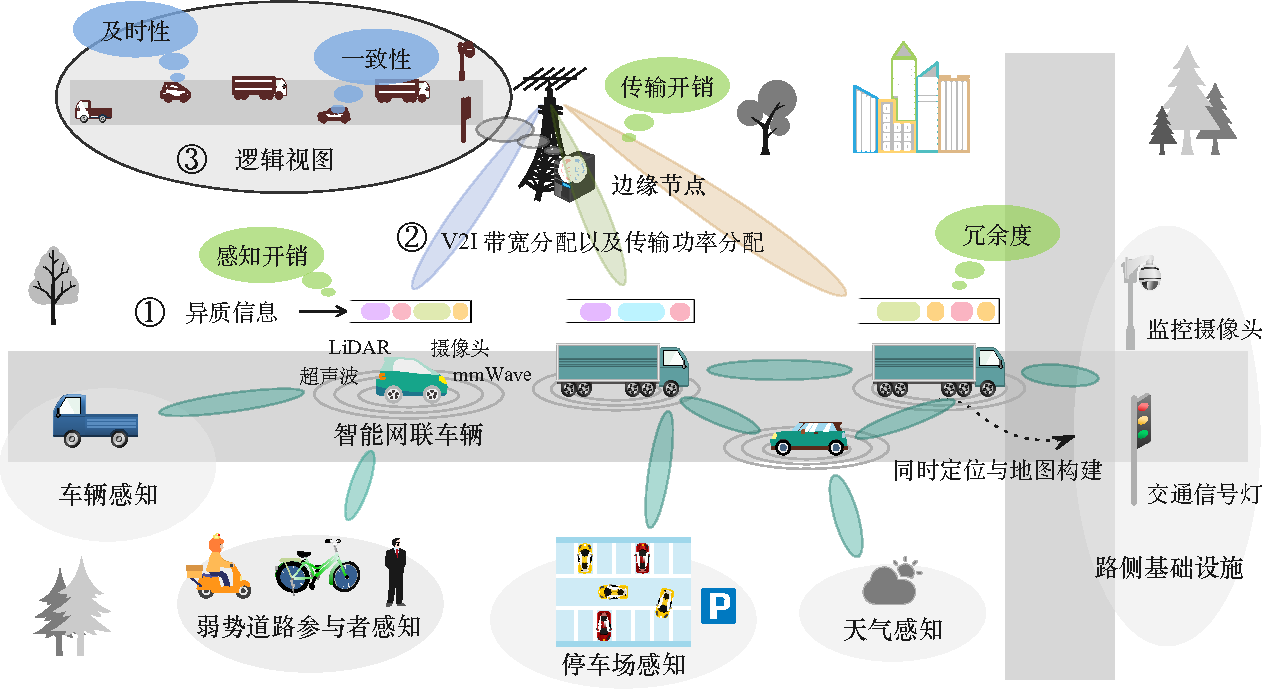
\includegraphics[width=0.38\textwidth]{fig/Fig4-1-architerture.pdf}
\end{figure}
\begin{figure}
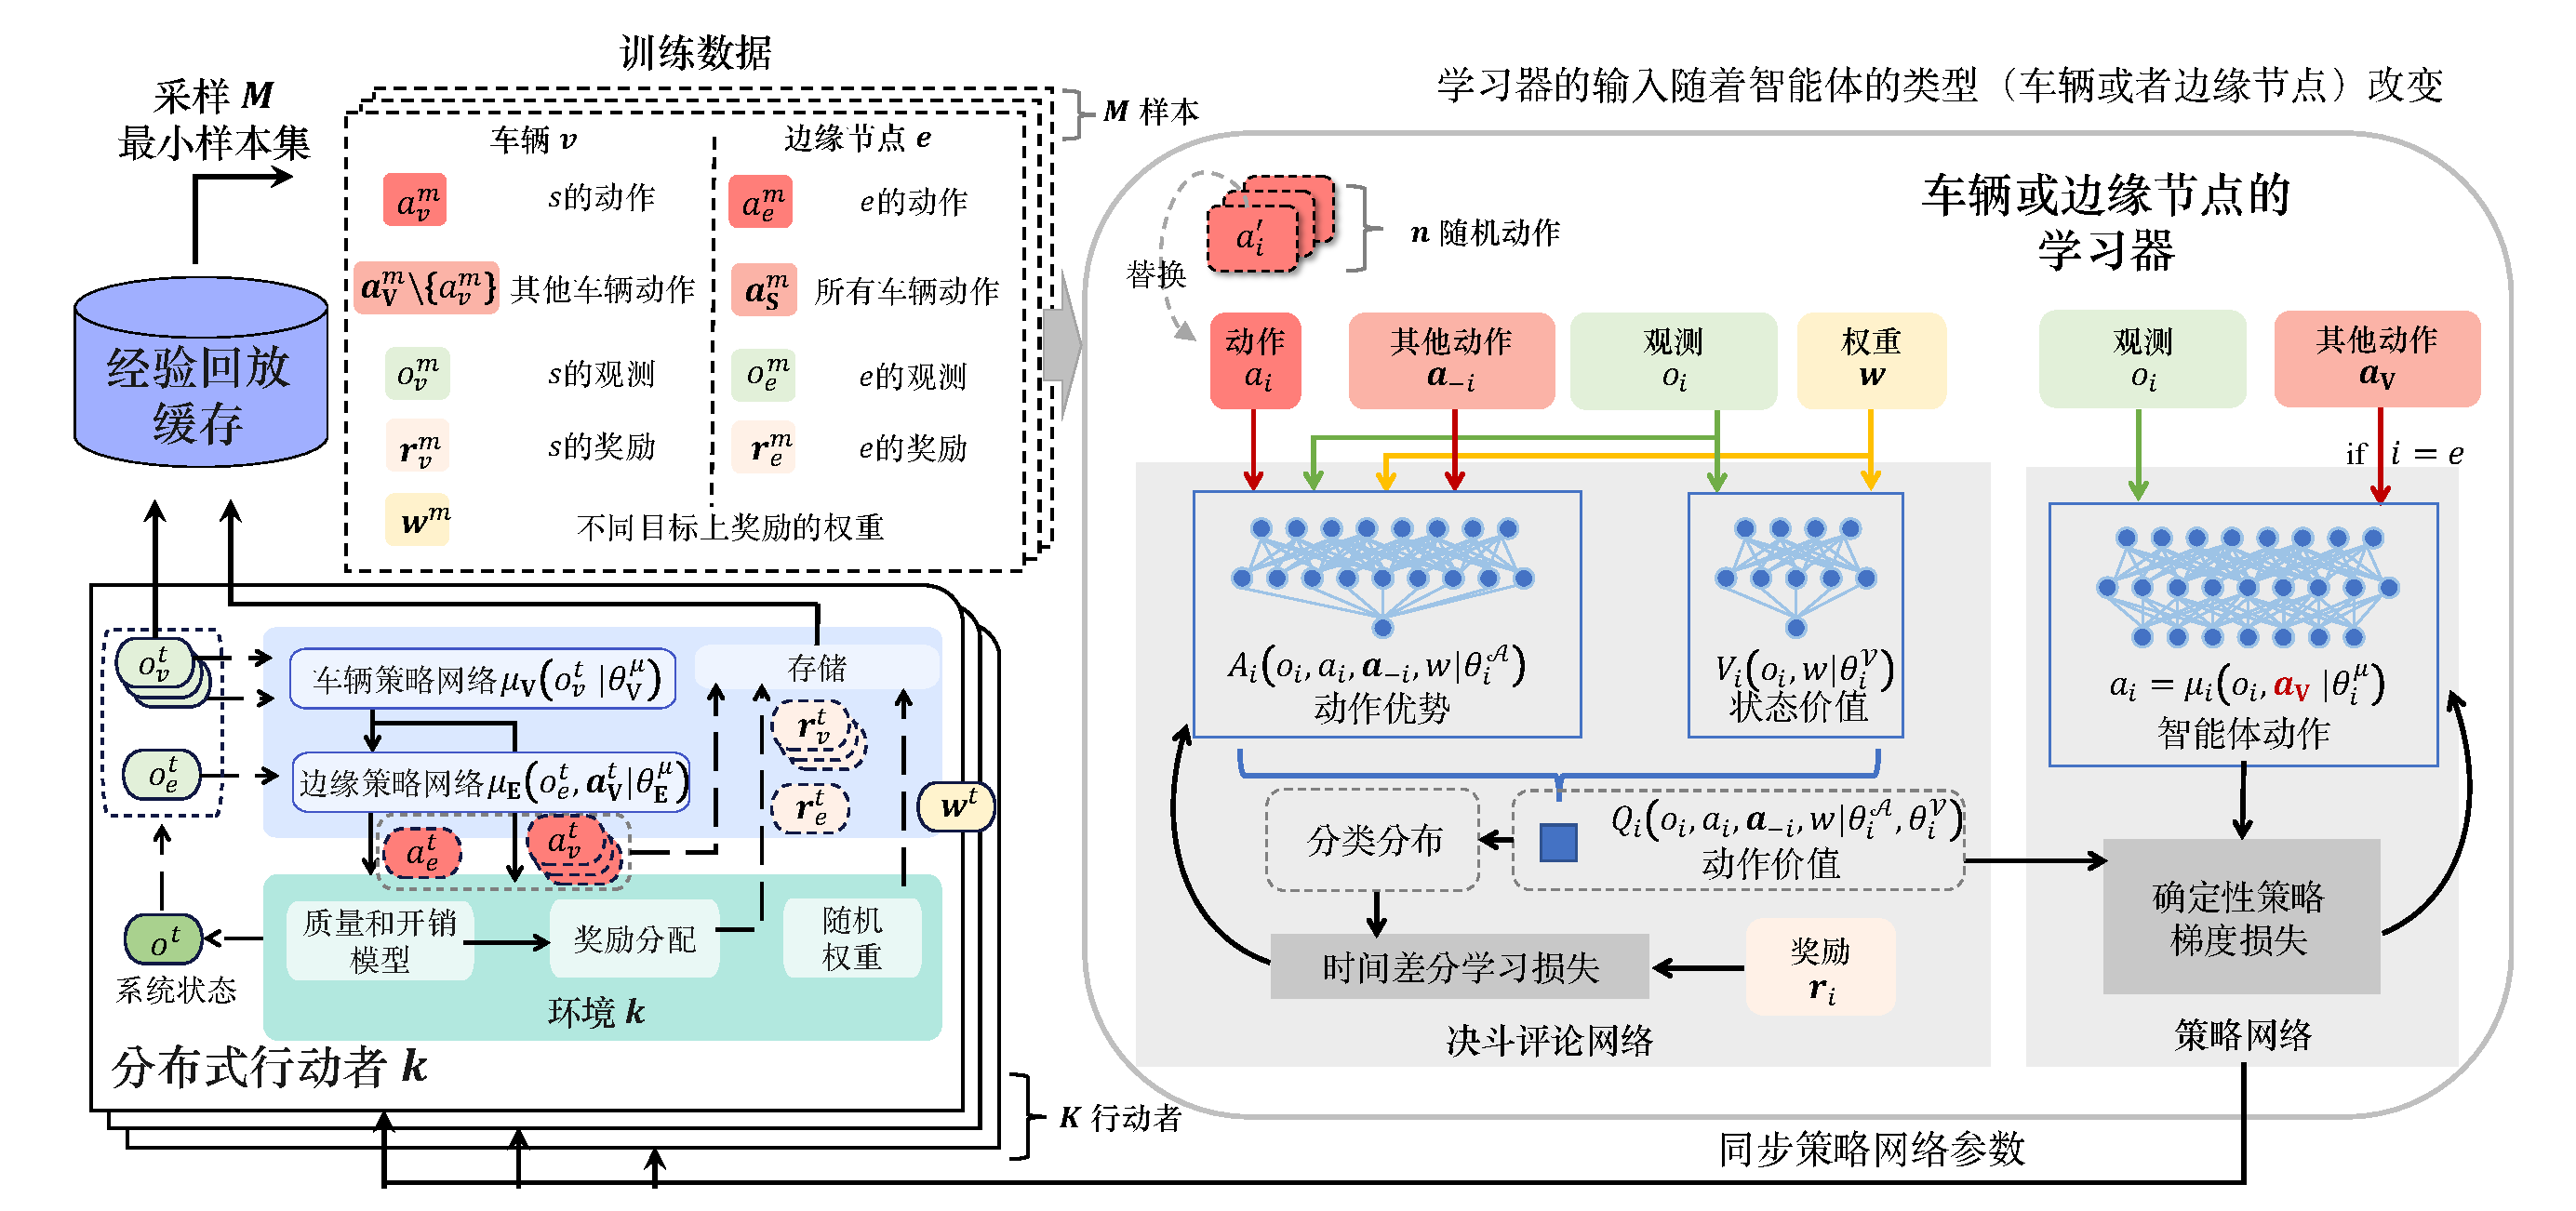
\includegraphics[width=0.38\textwidth]{fig/Fig4-2-solution-model.pdf}
\end{figure}
\end{textblock*}
\end{center}
\end{frame}

\begin{frame}{协同感知与 V2I 上传场景}
\frametitle{\englishfont \underline{问题}:逻辑视图构建场景}
\newBackground
\begin{center}
\begin{textblock*}{\textwidth}(3cm,2cm)
\begin{figure}
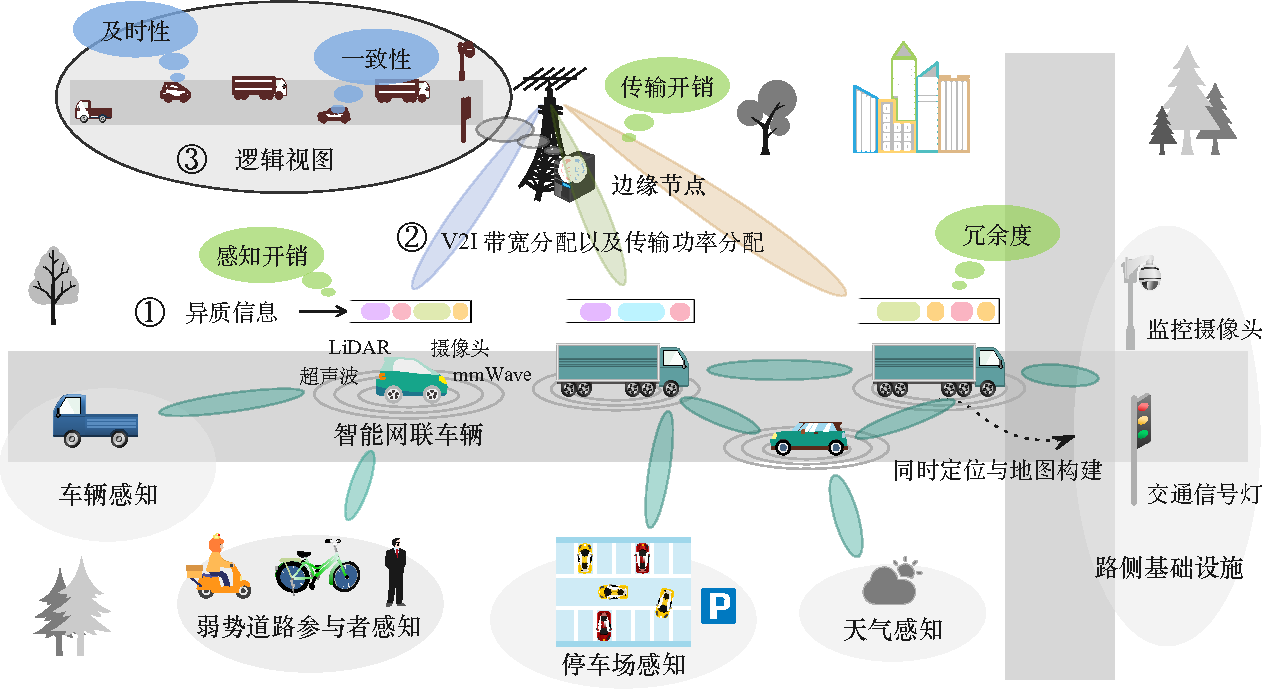
\includegraphics[width=0.75\textwidth]{fig/Fig4-1-architerture.pdf}
\end{figure}
\end{textblock*}
\end{center}

\begin{center}
\begin{textblock*}{\textwidth}(0.5cm,2cm)
\begin{itemize}[itemsep=0.2\baselineskip] \englishfont
		\item[\ding{111}] {\color{cqublue}{视图质量}}
		\begin{itemize}[itemsep=0.2\baselineskip] \small
			\item[\ding{226}] 及时性
			\item[\ding{226}] 一致性
		\end{itemize}
		\item[\ding{111}] {\color{cqublue}{视图开销}}
		\begin{itemize}[itemsep=0.2\baselineskip] \small
			\item[\ding{226}] 感知开销
			\item[\ding{226}] 传输开销
			\item[\ding{226}] 冗余度
		\end{itemize}
\end{itemize}
\end{textblock*}
\end{center}
\end{frame}

\begin{frame}
\newBackground
\frametitle{\englishfont \underline{问题}:VCPS 质量/开销模型}

\begin{overlayarea}{\textwidth}{3cm}
\only<1-1>{
\begin{center}
\begin{textblock*}{0.6\textwidth}(0cm,1.8cm)
\begin{equation}
	\mathscr{Q}=\frac{\sum_{\forall t \in \mathbf{T}} \sum_{\forall e \in \mathbf{E}} \sum_{\forall i \in \mathbf{I}_e^t} \operatorname{QV}_{i}}{\sum_{\forall t \in \mathbf{T}} \sum_{\forall e \in \mathbf{E}} |\mathbf{I}_e^t| } \notag
\end{equation}
\end{textblock*}
\end{center}
}

\only<1-4>{
\begin{center}
\begin{textblock*}{0.6\textwidth}(0cm,4.8cm)
\begin{equation}
	\mathscr{C}=\frac{\sum_{\forall t \in \mathbf{T}} \sum_{\forall e \in \mathbf{E}} \sum_{\forall i \in \mathbf{I}_e^t}  \operatorname{CV}_{i}}{\sum_{\forall t \in \mathbf{T}} \sum_{\forall e \in \mathbf{E}} |\mathbf{I}_e^t| } \notag
\end{equation}
\end{textblock*}
\end{center}
}

\only<2-2>{
\begin{center}
\begin{textblock*}{0.6\textwidth}(0cm,1.8cm)
\begin{equation}
	\mathscr{Q}=\frac{\sum_{\forall t \in \mathbf{T}} \sum_{\forall e \in \mathbf{E}} \sum_{\forall i \in \mathbf{I}_e^t} {\color{red}{\operatorname{QV}_{i}}}}{\sum_{\forall t \in \mathbf{T}} \sum_{\forall e \in \mathbf{E}} |\mathbf{I}_e^t| } \notag
\end{equation}
\end{textblock*}
\end{center}
}

\only<2-2>{
\begin{center}
\begin{textblock*}{0.6\textwidth}(0cm,1.8cm)
\begin{equation}
	\mathscr{Q}=\frac{\sum_{\forall t \in \mathbf{T}} \sum_{\forall e \in \mathbf{E}} \sum_{\forall i \in \mathbf{I}_e^t} {\color{red}{\operatorname{QV}_{i}}}}{\sum_{\forall t \in \mathbf{T}} \sum_{\forall e \in \mathbf{E}} |\mathbf{I}_e^t| } \notag
\end{equation}
\end{textblock*}
\end{center}
}

\only<2-2>{
\begin{center}
\begin{textblock*}{1\textwidth}(4.4cm,1.8cm)
视图质量
\begin{equation}
	{\color{red}{\operatorname{QV}_{i}}}= w_1 (1 -\hat{\Theta_{i}}) + w_2 (1 - \hat{\Psi_{i}}), \forall i \in \mathbf{I}_{e}^t, \forall e \in \mathbf{E} \notag
\end{equation}
\end{textblock*}
\end{center}
}

\only<3->{
\begin{center}
\begin{textblock*}{0.6\textwidth}(0cm,1.8cm)
\begin{equation}
	\mathscr{Q}=\frac{\sum_{\forall t \in \mathbf{T}} \sum_{\forall e \in \mathbf{E}} \sum_{\forall i \in \mathbf{I}_e^t} \operatorname{QV}_{i}}{\sum_{\forall t \in \mathbf{T}} \sum_{\forall e \in \mathbf{E}} |\mathbf{I}_e^t| } \notag
\end{equation}
\end{textblock*}
\end{center}
}

\only<3-3>{
\begin{center}
\begin{textblock*}{1\textwidth}(4.4cm,1.8cm)
视图质量
\begin{equation}
	\operatorname{QV}_{i}= w_1 (1 -{\color{red}{\hat{\Theta_{i}}}}) + w_2 (1 - \hat{\Psi_{i}}), \forall i \in \mathbf{I}_{e}^t, \forall e \in \mathbf{E} \notag
\end{equation}
\end{textblock*}
\end{center}
}

\only<3-3>{
\begin{center}
\begin{textblock*}{1\textwidth}(2.4cm,3.4cm)
{\color{red}{$\hat{\Theta_{i}}$}}:视图及时性
\end{textblock*}
\end{center}
}

\only<4->{
\begin{center}
\begin{textblock*}{1\textwidth}(2.4cm,3.4cm)
$\hat{\Theta_{i}}$:视图及时性
\end{textblock*}
\end{center}
}

\only<4-4>{
\begin{center}
\begin{textblock*}{1\textwidth}(4.4cm,1.8cm)
视图质量
\begin{equation}
	\operatorname{QV}_{i}= w_1 (1 -\hat{\Theta_{i}}) + w_2 (1 - {\color{red}{\hat{\Psi_{i}}}}), \forall i \in \mathbf{I}_{e}^t, \forall e \in \mathbf{E} \notag
\end{equation}
\end{textblock*}
\end{center}
}

\only<4-4>{
\begin{center}
\begin{textblock*}{1\textwidth}(6.4cm,3.4cm)
{\color{red}{$\hat{\Psi_{i}}$}}:视图一致性
\end{textblock*}
\end{center}
}

\only<5->{
\begin{center}
\begin{textblock*}{1\textwidth}(4.4cm,1.8cm)
视图质量
\begin{equation}
	\operatorname{QV}_{i}= w_1 (1 -\hat{\Theta_{i}}) + w_2 (1 - \hat{\Psi_{i}}), \forall i \in \mathbf{I}_{e}^t, \forall e \in \mathbf{E} \notag
\end{equation}
\end{textblock*}
\end{center}
}

\only<5->{
\begin{center}
\begin{textblock*}{1\textwidth}(6.4cm,3.4cm)
$\hat{\Psi_{i}}$:视图一致性
\end{textblock*}
\end{center}
}

\only<5-5>{
\begin{center}
\begin{textblock*}{0.6\textwidth}(0cm,4.8cm)
\begin{equation}
	\mathscr{C}=\frac{\sum_{\forall t \in \mathbf{T}} \sum_{\forall e \in \mathbf{E}} \sum_{\forall i \in \mathbf{I}_e^t}  {\color{red}{\operatorname{CV}_{i}}}}{\sum_{\forall t \in \mathbf{T}} \sum_{\forall e \in \mathbf{E}} |\mathbf{I}_e^t| } \notag
\end{equation}
\end{textblock*}
\end{center}
}

\only<5-5>{
\begin{center}
\begin{textblock*}{1\textwidth}(4.4cm,4.8cm)
视图开销
\begin{equation}
	{\color{red}{\operatorname{CV}_{i}}} = w_3  \hat{\Xi_{i}} +  w_4 \hat{\Phi_{i}} + w_5 \hat{\Omega_{i}}, \forall i \in \mathbf{I}_{e}^t, \forall e \in \mathbf{E} \notag
\end{equation}
\end{textblock*}
\end{center}
}

\only<6->{
\begin{center}
\begin{textblock*}{0.6\textwidth}(0cm,4.8cm)
\begin{equation}
	\mathscr{C}=\frac{\sum_{\forall t \in \mathbf{T}} \sum_{\forall e \in \mathbf{E}} \sum_{\forall i \in \mathbf{I}_e^t}  \operatorname{CV}_{i}}{\sum_{\forall t \in \mathbf{T}} \sum_{\forall e \in \mathbf{E}} |\mathbf{I}_e^t| } \notag
\end{equation}
\end{textblock*}
\end{center}
}

\only<6-6>{
\begin{center}
\begin{textblock*}{1\textwidth}(4.4cm,4.8cm)
视图开销
\begin{equation}
	\operatorname{CV}_{i} = w_3  {\color{red}{\hat{\Xi_{i}}}} +  w_4 \hat{\Phi_{i}} + w_5 \hat{\Omega_{i}}, \forall i \in \mathbf{I}_{e}^t, \forall e \in \mathbf{E} \notag
\end{equation}
\end{textblock*}
\end{center}
}

\only<6-6>{
\begin{center}
\begin{textblock*}{1\textwidth}(2.4cm,6.4cm)
{\color{red}{$\hat{\Xi_{i}}$}}:视图冗余度
\end{textblock*}
\end{center}
}

\only<7->{
\begin{center}
\begin{textblock*}{1\textwidth}(2.4cm,6.4cm)
$\hat{\Xi_{i}}$:视图冗余度
\end{textblock*}
\end{center}
}

\only<7-7>{
\begin{center}
\begin{textblock*}{1\textwidth}(4.4cm,4.8cm)
视图开销
\begin{equation}
	\operatorname{CV}_{i} = w_3 \hat{\Xi_{i}} +  w_4 {\color{red}{\hat{\Phi_{i}}}} + w_5 \hat{\Omega_{i}}, \forall i \in \mathbf{I}_{e}^t, \forall e \in \mathbf{E} \notag
\end{equation}
\end{textblock*}
\end{center}
}

\only<7-7>{
\begin{center}
\begin{textblock*}{1\textwidth}(6.4cm,6.4cm)
{\color{red}{$\hat{\Phi_{i}}$}}:视图感知开销
\end{textblock*}
\end{center}
}

\only<8->{
\begin{center}
\begin{textblock*}{1\textwidth}(6.4cm,6.4cm)
$\hat{\Phi_{i}}$:视图感知开销
\end{textblock*}
\end{center}
}

\only<8-8>{
\begin{center}
\begin{textblock*}{1\textwidth}(4.4cm,4.8cm)
视图开销
\begin{equation}
	\operatorname{CV}_{i} = w_3 \hat{\Xi_{i}} +  w_4 \hat{\Phi_{i}} + w_5 {\color{red}{\hat{\Omega_{i}}}}, \forall i \in \mathbf{I}_{e}^t, \forall e \in \mathbf{E} \notag
\end{equation}
\end{textblock*}
\end{center}
}

\only<8-8>{
\begin{center}
\begin{textblock*}{1\textwidth}(4.4cm,7.4cm)
{\color{red}{$\hat{\Omega_{i}}$}}:视图传输开销
\end{textblock*}
\end{center}
}

\end{overlayarea}

\begin{center}
\begin{textblock*}{0.6\textwidth}(1cm,1.8cm)
\begin{itemize} \englishfont
	\item[\ding{111}]  {\color{cqublue}{VCPS 质量模型}}
	\item
	\item
	\item
	\item
	\item[\ding{111}]  {\color{cqublue}{VCPS开销模型}}
\end{itemize}
\end{textblock*}
\end{center}

\end{frame}

\begin{frame}
\frametitle{\englishfont \underline{问题}:双目标优化问题}
\newBackground

\begin{overlayarea}{\textwidth}{3cm}
\only<1-1>{
\begin{center}
\begin{textblock*}{1\textwidth}(0.5cm,1.6cm)
\begin{align}
	\mathcal{P}4.1: & \max_{\mathbf{C}, \boldsymbol{\Lambda}, \mathbf{P}, \boldsymbol{\Pi}, \mathbf{B}} \mathscr{Q}, \min_{\mathbf{C}, \boldsymbol{\Lambda}, \mathbf{P}, \boldsymbol{\Pi}, \mathbf{B}} \mathscr{C} \notag \\
	\text { s.t. }
	& (4.1) \sim (4.5) \notag \\
    &\mathcal{C}4.1: \sum_{\forall d \subseteq \mathbf{D}_v^t} \lambda_{d, v}^{t} \mu_d<1,\ \forall v \in \mathbf{V}, \forall t \in \mathbf{T} \notag \\
    &\mathcal{C}4.2: \inf_{\mathbb{P} \in \tilde{p}} \operatorname{Pr}_{[\mathbb{P}]}\left(\operatorname{SNR}_{v, e}^{t} \geq \operatorname{SNR}_{v, e}^{\operatorname{tgt}}\right) \geq \delta, \forall v \in \mathbf{V}, \forall t \in \mathbf{T} \notag \\
    &\mathcal{C}4.3: {\sum_{\forall v \in \mathbf{V}_e^{t}}b_v^t} \leq b_e, \forall t \in \mathbf{T} \notag
\end{align}
\end{textblock*}
\end{center}
}

\only<2-2>{
\begin{center}
\begin{textblock*}{1\textwidth}(0.5cm,1.6cm)
\begin{align}
	\mathcal{P}4.2: & \max_{ \mathbf{C}, \boldsymbol{\Lambda}, \mathbf{P}, \boldsymbol{\Pi}, \mathbf{B} } \left (\mathscr{Q}, {\color{red}{\mathscr{P}}} \right )  \notag \\
	\text { s.t. }
	& (4.1) \sim (4.5) \notag \\
    &\mathcal{C}4.1: \sum_{\forall d \subseteq \mathbf{D}_v^t} \lambda_{d, v}^{t} \mu_d<1,\ \forall v \in \mathbf{V}, \forall t \in \mathbf{T} \notag \\
    &\mathcal{C}4.2: \inf_{\mathbb{P} \in \tilde{p}} \operatorname{Pr}_{[\mathbb{P}]}\left(\operatorname{SNR}_{v, e}^{t} \geq \operatorname{SNR}_{v, e}^{\operatorname{tgt}}\right) \geq \delta, \forall v \in \mathbf{V}, \forall t \in \mathbf{T} \notag \\
    &\mathcal{C}4.3: {\sum_{\forall v \in \mathbf{V}_e^{t}}b_v^t} \leq b_e, \forall t \in \mathbf{T} \notag
\end{align}
\end{textblock*}
\end{center}
}

\only<2-2>{
\begin{center}
\begin{textblock*}{1\textwidth}(0.5cm,7.1cm) \englishfont
{\color{red}{$\mathscr{P}$}}:VCPS 利润 $\mathscr{P}= \frac{\sum_{\forall t \in \mathbf{T}} \sum_{\forall e \in \mathbf{E}} \sum_{\forall i \in \mathbf{I}_e^t}   \operatorname{PV}_{j} }{\sum_{\forall t \in \mathbf{T}} \sum_{\forall e \in \mathbf{E}} |\mathbf{I}_e^t| }$
\end{textblock*}
\end{center}
}


\only<3-3>{
\begin{center}
\begin{textblock*}{1\textwidth}(0.5cm,1.6cm)
\begin{align}
	\mathcal{P}4.2: & \max_{ {\color{red}{\mathbf{C}}}, \boldsymbol{\Lambda}, \mathbf{P}, \boldsymbol{\Pi}, \mathbf{B} } \left (\mathscr{Q}, \mathscr{P} \right )  \notag \\
	\text { s.t. }
	& (4.1) \sim (4.5) \notag \\
    &\mathcal{C}4.1: \sum_{\forall d \subseteq \mathbf{D}_v^t} \lambda_{d, v}^{t} \mu_d<1,\ \forall v \in \mathbf{V}, \forall t \in \mathbf{T} \notag \\
    &\mathcal{C}4.2: \inf_{\mathbb{P} \in \tilde{p}} \operatorname{Pr}_{[\mathbb{P}]}\left(\operatorname{SNR}_{v, e}^{t} \geq \operatorname{SNR}_{v, e}^{\operatorname{tgt}}\right) \geq \delta, \forall v \in \mathbf{V}, \forall t \in \mathbf{T} \notag \\
    &\mathcal{C}4.3: {\sum_{\forall v \in \mathbf{V}_e^{t}}b_v^t} \leq b_e, \forall t \in \mathbf{T} \notag
\end{align}
\end{textblock*}
\end{center}
}

\only<3-3>{
\begin{center}
\begin{textblock*}{1\textwidth}(0.5cm,7.1cm) \englishfont
{\color{red}{$\mathbf{C}$}}:感知信息决策 $\mathbf{C} = \left \{ c_{d, v}^t \vert \forall d \in \mathbf{D}_{v}, \forall v \in \mathbf{V}, \forall t \in \mathbf{T} \right  \}$
\end{textblock*}
\end{center}
}

\only<4-4>{
\begin{center}
\begin{textblock*}{1\textwidth}(0.5cm,1.6cm)
\begin{align}
	\mathcal{P}4.2: & \max_{ \mathbf{C}, {\color{red}{\boldsymbol{\Lambda}}}, \mathbf{P}, \boldsymbol{\Pi}, \mathbf{B} } \left (\mathscr{Q}, \mathscr{P} \right )  \notag \\
	\text { s.t. }
	& (4.1) \sim (4.5) \notag \\
    &\mathcal{C}4.1: \sum_{\forall d \subseteq \mathbf{D}_v^t} \lambda_{d, v}^{t} \mu_d<1,\ \forall v \in \mathbf{V}, \forall t \in \mathbf{T} \notag \\
    &\mathcal{C}4.2: \inf_{\mathbb{P} \in \tilde{p}} \operatorname{Pr}_{[\mathbb{P}]}\left(\operatorname{SNR}_{v, e}^{t} \geq \operatorname{SNR}_{v, e}^{\operatorname{tgt}}\right) \geq \delta, \forall v \in \mathbf{V}, \forall t \in \mathbf{T} \notag \\
    &\mathcal{C}4.3: {\sum_{\forall v \in \mathbf{V}_e^{t}}b_v^t} \leq b_e, \forall t \in \mathbf{T} \notag
\end{align}
\end{textblock*}
\end{center}
}

\only<4-4>{
\begin{center}
\begin{textblock*}{1\textwidth}(0.5cm,7.1cm) \englishfont
{\color{red}{$\boldsymbol{\Lambda}$}}:感知频率 $\boldsymbol{\Lambda} = \left \{ \lambda_{d, v}^{t} \vert \forall d \in \mathbf{D}_v^t  , \forall v \in \mathbf{V}, \forall t \in \mathbf{T} \right \}$
\end{textblock*}
\end{center}
}

\only<5-5>{
\begin{center}
\begin{textblock*}{1\textwidth}(0.5cm,1.6cm)
\begin{align}
	\mathcal{P}4.2: & \max_{ \mathbf{C}, \boldsymbol{\Lambda}, {\color{red}{\mathbf{P}}}, \boldsymbol{\Pi}, \mathbf{B} } \left (\mathscr{Q}, \mathscr{P} \right )  \notag \\
	\text { s.t. }
	& (4.1) \sim (4.5) \notag \\
    &\mathcal{C}4.1: \sum_{\forall d \subseteq \mathbf{D}_v^t} \lambda_{d, v}^{t} \mu_d<1,\ \forall v \in \mathbf{V}, \forall t \in \mathbf{T} \notag \\
    &\mathcal{C}4.2: \inf_{\mathbb{P} \in \tilde{p}} \operatorname{Pr}_{[\mathbb{P}]}\left(\operatorname{SNR}_{v, e}^{t} \geq \operatorname{SNR}_{v, e}^{\operatorname{tgt}}\right) \geq \delta, \forall v \in \mathbf{V}, \forall t \in \mathbf{T} \notag \\
    &\mathcal{C}4.3: {\sum_{\forall v \in \mathbf{V}_e^{t}}b_v^t} \leq b_e, \forall t \in \mathbf{T} \notag
\end{align}
\end{textblock*}
\end{center}
}

\only<5-5>{
\begin{center}
\begin{textblock*}{1\textwidth}(0.5cm,7.1cm) \englishfont
{\color{red}{$\mathbf{P}$}}:上传优先级 $\mathbf{P} = \left \{ p_{d, v}^{t} \vert \forall d \in \mathbf{D}_v^t  , \forall v \in \mathbf{V}, \forall t \in \mathbf{T}\right \}$
\end{textblock*}
\end{center}
}

\only<6-6>{
\begin{center}
\begin{textblock*}{1\textwidth}(0.5cm,1.6cm)
\begin{align}
	\mathcal{P}4.2: & \max_{ \mathbf{C}, \boldsymbol{\Lambda}, \mathbf{P}, {\color{red}{\boldsymbol{\Pi}}}, \mathbf{B} } \left (\mathscr{Q}, \mathscr{P} \right )  \notag \\
	\text { s.t. }
	& (4.1) \sim (4.5) \notag \\
    &\mathcal{C}4.1: \sum_{\forall d \subseteq \mathbf{D}_v^t} \lambda_{d, v}^{t} \mu_d<1,\ \forall v \in \mathbf{V}, \forall t \in \mathbf{T} \notag \\
    &\mathcal{C}4.2: \inf_{\mathbb{P} \in \tilde{p}} \operatorname{Pr}_{[\mathbb{P}]}\left(\operatorname{SNR}_{v, e}^{t} \geq \operatorname{SNR}_{v, e}^{\operatorname{tgt}}\right) \geq \delta, \forall v \in \mathbf{V}, \forall t \in \mathbf{T} \notag \\
    &\mathcal{C}4.3: {\sum_{\forall v \in \mathbf{V}_e^{t}}b_v^t} \leq b_e, \forall t \in \mathbf{T} \notag
\end{align}
\end{textblock*}
\end{center}
}

\only<6-6>{
\begin{center}
\begin{textblock*}{1\textwidth}(0.5cm,7.1cm) \englishfont
{\color{red}{$\boldsymbol{\Pi}$}}:传输功率 $\boldsymbol{\Pi} = \left \{ \pi_v^t \vert \forall v \in \mathbf{V}, \forall t \in \mathbf{T} \right \}$
\end{textblock*}
\end{center}
}

\only<7-7>{
\begin{center}
\begin{textblock*}{1\textwidth}(0.5cm,1.6cm)
\begin{align}
	\mathcal{P}4.2: & \max_{ \mathbf{C}, \boldsymbol{\Lambda}, \mathbf{P}, \boldsymbol{\Pi}, {\color{red}{\mathbf{B}}} } \left (\mathscr{Q}, \mathscr{P} \right )  \notag \\
	\text { s.t. }
	& (4.1) \sim (4.5) \notag \\
    &\mathcal{C}4.1: \sum_{\forall d \subseteq \mathbf{D}_v^t} \lambda_{d, v}^{t} \mu_d<1,\ \forall v \in \mathbf{V}, \forall t \in \mathbf{T} \notag \\
    &\mathcal{C}4.2: \inf_{\mathbb{P} \in \tilde{p}} \operatorname{Pr}_{[\mathbb{P}]}\left(\operatorname{SNR}_{v, e}^{t} \geq \operatorname{SNR}_{v, e}^{\operatorname{tgt}}\right) \geq \delta, \forall v \in \mathbf{V}, \forall t \in \mathbf{T} \notag \\
    &\mathcal{C}4.3: {\sum_{\forall v \in \mathbf{V}_e^{t}}b_v^t} \leq b_e, \forall t \in \mathbf{T} \notag
\end{align}
\end{textblock*}
\end{center}
}

\only<7-7>{
\begin{center}
\begin{textblock*}{1\textwidth}(0.5cm,7.1cm) \englishfont
{\color{red}{$\mathbf{B}$}}:V2I带宽分配 $\mathbf{B} = \left \{ b_v^t \vert \forall v \in \mathbf{V}, \forall t \in \mathbf{T}\right \}$
\end{textblock*}
\end{center}
}

\only<8-8>{
\begin{center}
\begin{textblock*}{1\textwidth}(0.5cm,1.6cm)
\begin{align}
	\mathcal{P}4.2: & \max_{ \mathbf{C}, \boldsymbol{\Lambda}, \mathbf{P}, \boldsymbol{\Pi}, \mathbf{B} } \left (\mathscr{Q}, \mathscr{P} \right )  \notag \\
	\text { s.t. }
	& {\color{red}{(4.1) \sim (4.5)}} \notag \\
    &\mathcal{C}4.1: \sum_{\forall d \subseteq \mathbf{D}_v^t} \lambda_{d, v}^{t} \mu_d<1,\ \forall v \in \mathbf{V}, \forall t \in \mathbf{T} \notag \\
    &\mathcal{C}4.2: \inf_{\mathbb{P} \in \tilde{p}} \operatorname{Pr}_{[\mathbb{P}]}\left(\operatorname{SNR}_{v, e}^{t} \geq \operatorname{SNR}_{v, e}^{\operatorname{tgt}}\right) \geq \delta, \forall v \in \mathbf{V}, \forall t \in \mathbf{T} \notag \\
    &\mathcal{C}4.3: {\sum_{\forall v \in \mathbf{V}_e^{t}}b_v^t} \leq b_e, \forall t \in \mathbf{T} \notag
\end{align}
\end{textblock*}
\end{center}
}

\only<8-8>{
\begin{center}
\begin{textblock*}{1\textwidth}(0.5cm,7.1cm) \englishfont
{\color{red}{$(4.1) \sim (4.5)$}}:决策变量取值范围限制
\end{textblock*}
\end{center}
}

\only<9-9>{
\begin{center}
\begin{textblock*}{1\textwidth}(0.5cm,1.6cm)
\begin{align}
	\mathcal{P}4.2: & \max_{ \mathbf{C}, \boldsymbol{\Lambda}, \mathbf{P}, \boldsymbol{\Pi}, \mathbf{B} } \left (\mathscr{Q}, \mathscr{P} \right )  \notag \\
	\text { s.t. }
	& (4.1) \sim (4.5) \notag \\
    &{\color{red}{\mathcal{C}4.1}}: \sum_{\forall d \subseteq \mathbf{D}_v^t} \lambda_{d, v}^{t} \mu_d<1,\ \forall v \in \mathbf{V}, \forall t \in \mathbf{T} \notag \\
    &\mathcal{C}4.2: \inf_{\mathbb{P} \in \tilde{p}} \operatorname{Pr}_{[\mathbb{P}]}\left(\operatorname{SNR}_{v, e}^{t} \geq \operatorname{SNR}_{v, e}^{\operatorname{tgt}}\right) \geq \delta, \forall v \in \mathbf{V}, \forall t \in \mathbf{T} \notag \\
    &\mathcal{C}4.3: {\sum_{\forall v \in \mathbf{V}_e^{t}}b_v^t} \leq b_e, \forall t \in \mathbf{T} \notag
\end{align}
\end{textblock*}
\end{center}
}

\only<9-9>{
\begin{center}
\begin{textblock*}{1\textwidth}(0.5cm,7.1cm) \englishfont
{\color{red}{$\mathcal{C}4.1$}}:保证队列稳定状态
\end{textblock*}
\end{center}
}

\only<10-10>{
\begin{center}
\begin{textblock*}{1\textwidth}(0.5cm,1.6cm)
\begin{align}
	\mathcal{P}4.2: & \max_{ \mathbf{C}, \boldsymbol{\Lambda}, \mathbf{P}, \boldsymbol{\Pi}, \mathbf{B} } \left (\mathscr{Q}, \mathscr{P} \right )  \notag \\
	\text { s.t. }
	& (4.1) \sim (4.5) \notag \\
    &\mathcal{C}4.1: \sum_{\forall d \subseteq \mathbf{D}_v^t} \lambda_{d, v}^{t} \mu_d<1,\ \forall v \in \mathbf{V}, \forall t \in \mathbf{T} \notag \\
    &{\color{red}{\mathcal{C}4.2}}: \inf_{\mathbb{P} \in \tilde{p}} \operatorname{Pr}_{[\mathbb{P}]}\left(\operatorname{SNR}_{v, e}^{t} \geq \operatorname{SNR}_{v, e}^{\operatorname{tgt}}\right) \geq \delta, \forall v \in \mathbf{V}, \forall t \in \mathbf{T} \notag \\
    &\mathcal{C}4.3: {\sum_{\forall v \in \mathbf{V}_e^{t}}b_v^t} \leq b_e, \forall t \in \mathbf{T} \notag
\end{align}
\end{textblock*}
\end{center}
}

\only<10-10>{
\begin{center}
\begin{textblock*}{1\textwidth}(0.5cm,7.1cm) \englishfont
{\color{red}{$\mathcal{C}4.2$}}:保证传输可靠性
\end{textblock*}
\end{center}
}

\only<11-11>{
\begin{center}
\begin{textblock*}{1\textwidth}(0.5cm,1.6cm)
\begin{align}
	\mathcal{P}4.2: & \max_{ \mathbf{C}, \boldsymbol{\Lambda}, \mathbf{P}, \boldsymbol{\Pi}, \mathbf{B} } \left (\mathscr{Q}, \mathscr{P} \right )  \notag \\
	\text { s.t. }
	& (4.1) \sim (4.5) \notag \\
    &\mathcal{C}4.1: \sum_{\forall d \subseteq \mathbf{D}_v^t} \lambda_{d, v}^{t} \mu_d<1,\ \forall v \in \mathbf{V}, \forall t \in \mathbf{T} \notag \\
    &\mathcal{C}4.2: \inf_{\mathbb{P} \in \tilde{p}} \operatorname{Pr}_{[\mathbb{P}]}\left(\operatorname{SNR}_{v, e}^{t} \geq \operatorname{SNR}_{v, e}^{\operatorname{tgt}}\right) \geq \delta, \forall v \in \mathbf{V}, \forall t \in \mathbf{T} \notag \\
    &{\color{red}{\mathcal{C}4.3}}: {\sum_{\forall v \in \mathbf{V}_e^{t}}b_v^t} \leq b_e, \forall t \in \mathbf{T} \notag
\end{align}
\end{textblock*}
\end{center}
}

\only<11-11>{
\begin{center}
\begin{textblock*}{1\textwidth}(0.5cm,7.1cm) \englishfont
{\color{red}{$\mathcal{C}4.3$}}:边缘节点$e$分配的V2I带宽之和不能超过其容量$b_e$
\end{textblock*}
\end{center}
}

\end{overlayarea}
\end{frame}


\begin{frame}
\frametitle{\englishfont \underline{算法}:流程}
\newBackground
\begin{center}
\begin{textblock*}{\textwidth}(4.5cm,2.6cm)
\begin{figure}
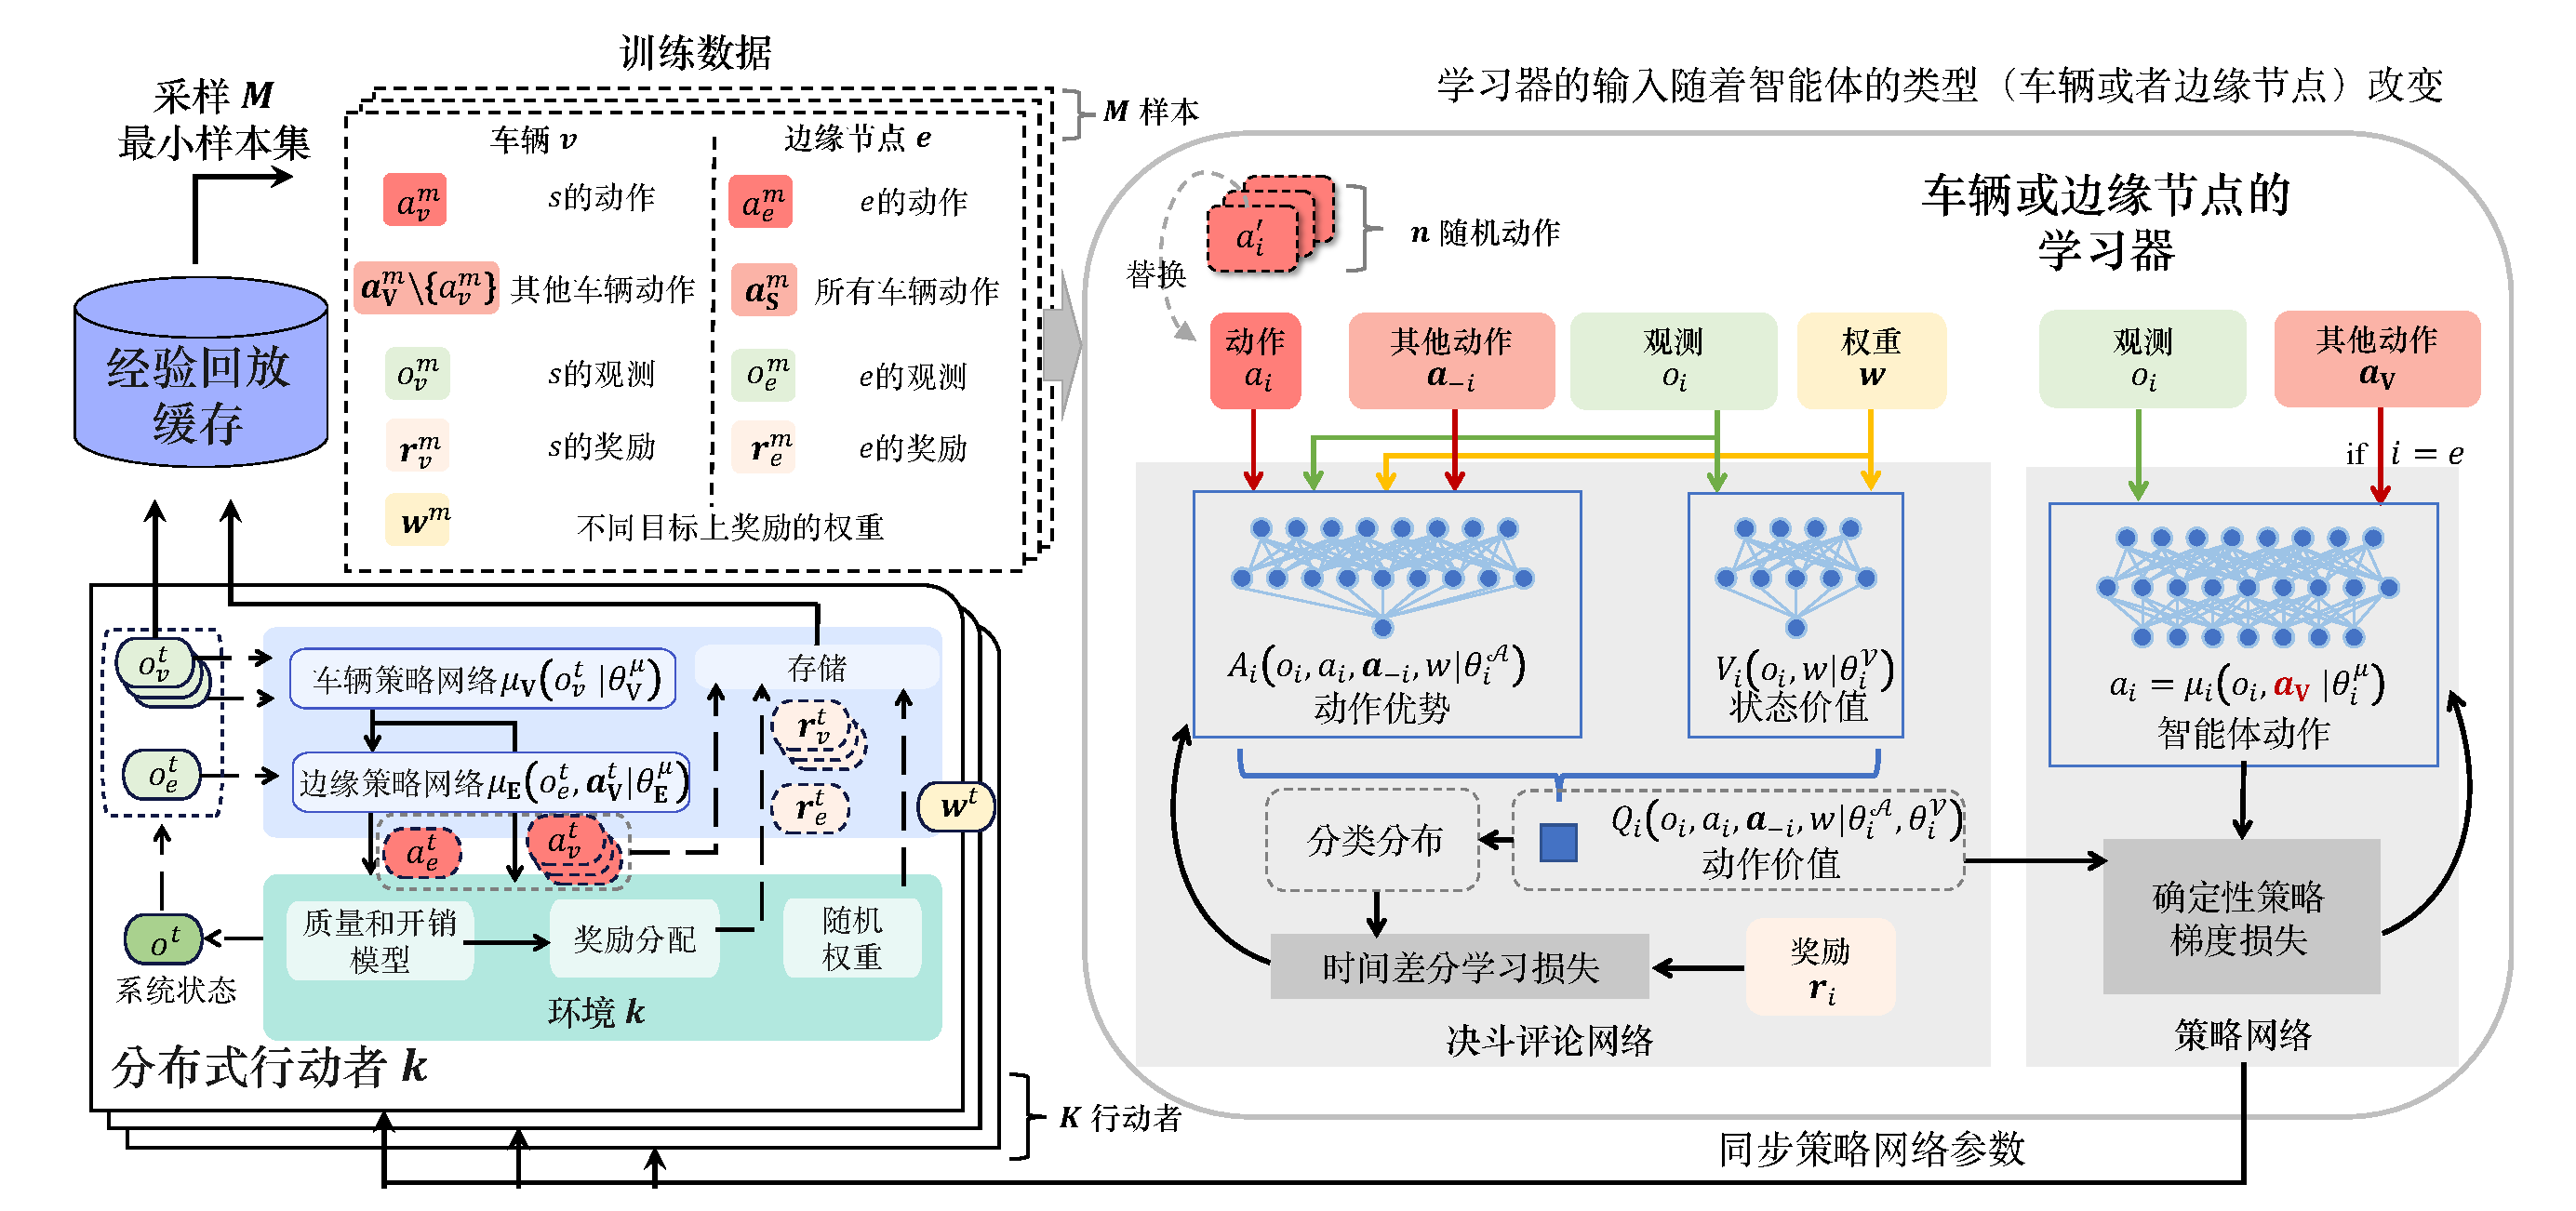
\includegraphics[width=0.65\textwidth]{fig/Fig4-2-solution-model.pdf}
\end{figure}
\end{textblock*}
\end{center}

\begin{center}
\begin{textblock*}{0.45\textwidth}(0.5cm,1.8cm)
\begin{itemize}[itemsep=0.2\baselineskip] \englishfont 
	\item[\ding{111}] {\color{cqublue}{初始化}}
	\begin{itemize}[itemsep=0.2\baselineskip]
	\begin{small}
		\item[\ding{226}] 网络参数、经验回放缓存
	\end{small}
	\end{itemize}
	\item[\ding{111}] {\color{cqublue}{分布式策略执行}}
	\begin{itemize}[itemsep=0.2\baselineskip]
	\begin{small}
		\item[\ding{226}] $K$分布式行动者启动
		\item[\ding{226}] 独立与环境交互,并存储经验
		\item[\ding{226}] 交互过程将持续到学习器训练过程结束
	\end{small}
	\end{itemize}
	\item[\ding{111}] {\color{cqublue}{网络学习与更新}}
	\begin{itemize}[itemsep=0.2\baselineskip]
	\begin{small}
		\item[\ding{226}] 抽取小批量训练样本
		\item[\ding{226}] 评论家网络:基于分类分布的时间差分学习
		\item[\ding{226}] 策略网络:策略梯度
	\end{small}
	\end{itemize}
\end{itemize}
\end{textblock*}
\end{center}

\end{frame}

\begin{frame}
\frametitle{\englishfont \underline{算法}:MAMO模型}
\newBackground
\begin{center}
\begin{textblock*}{\textwidth}(4.5cm,2.6cm)
\begin{figure}
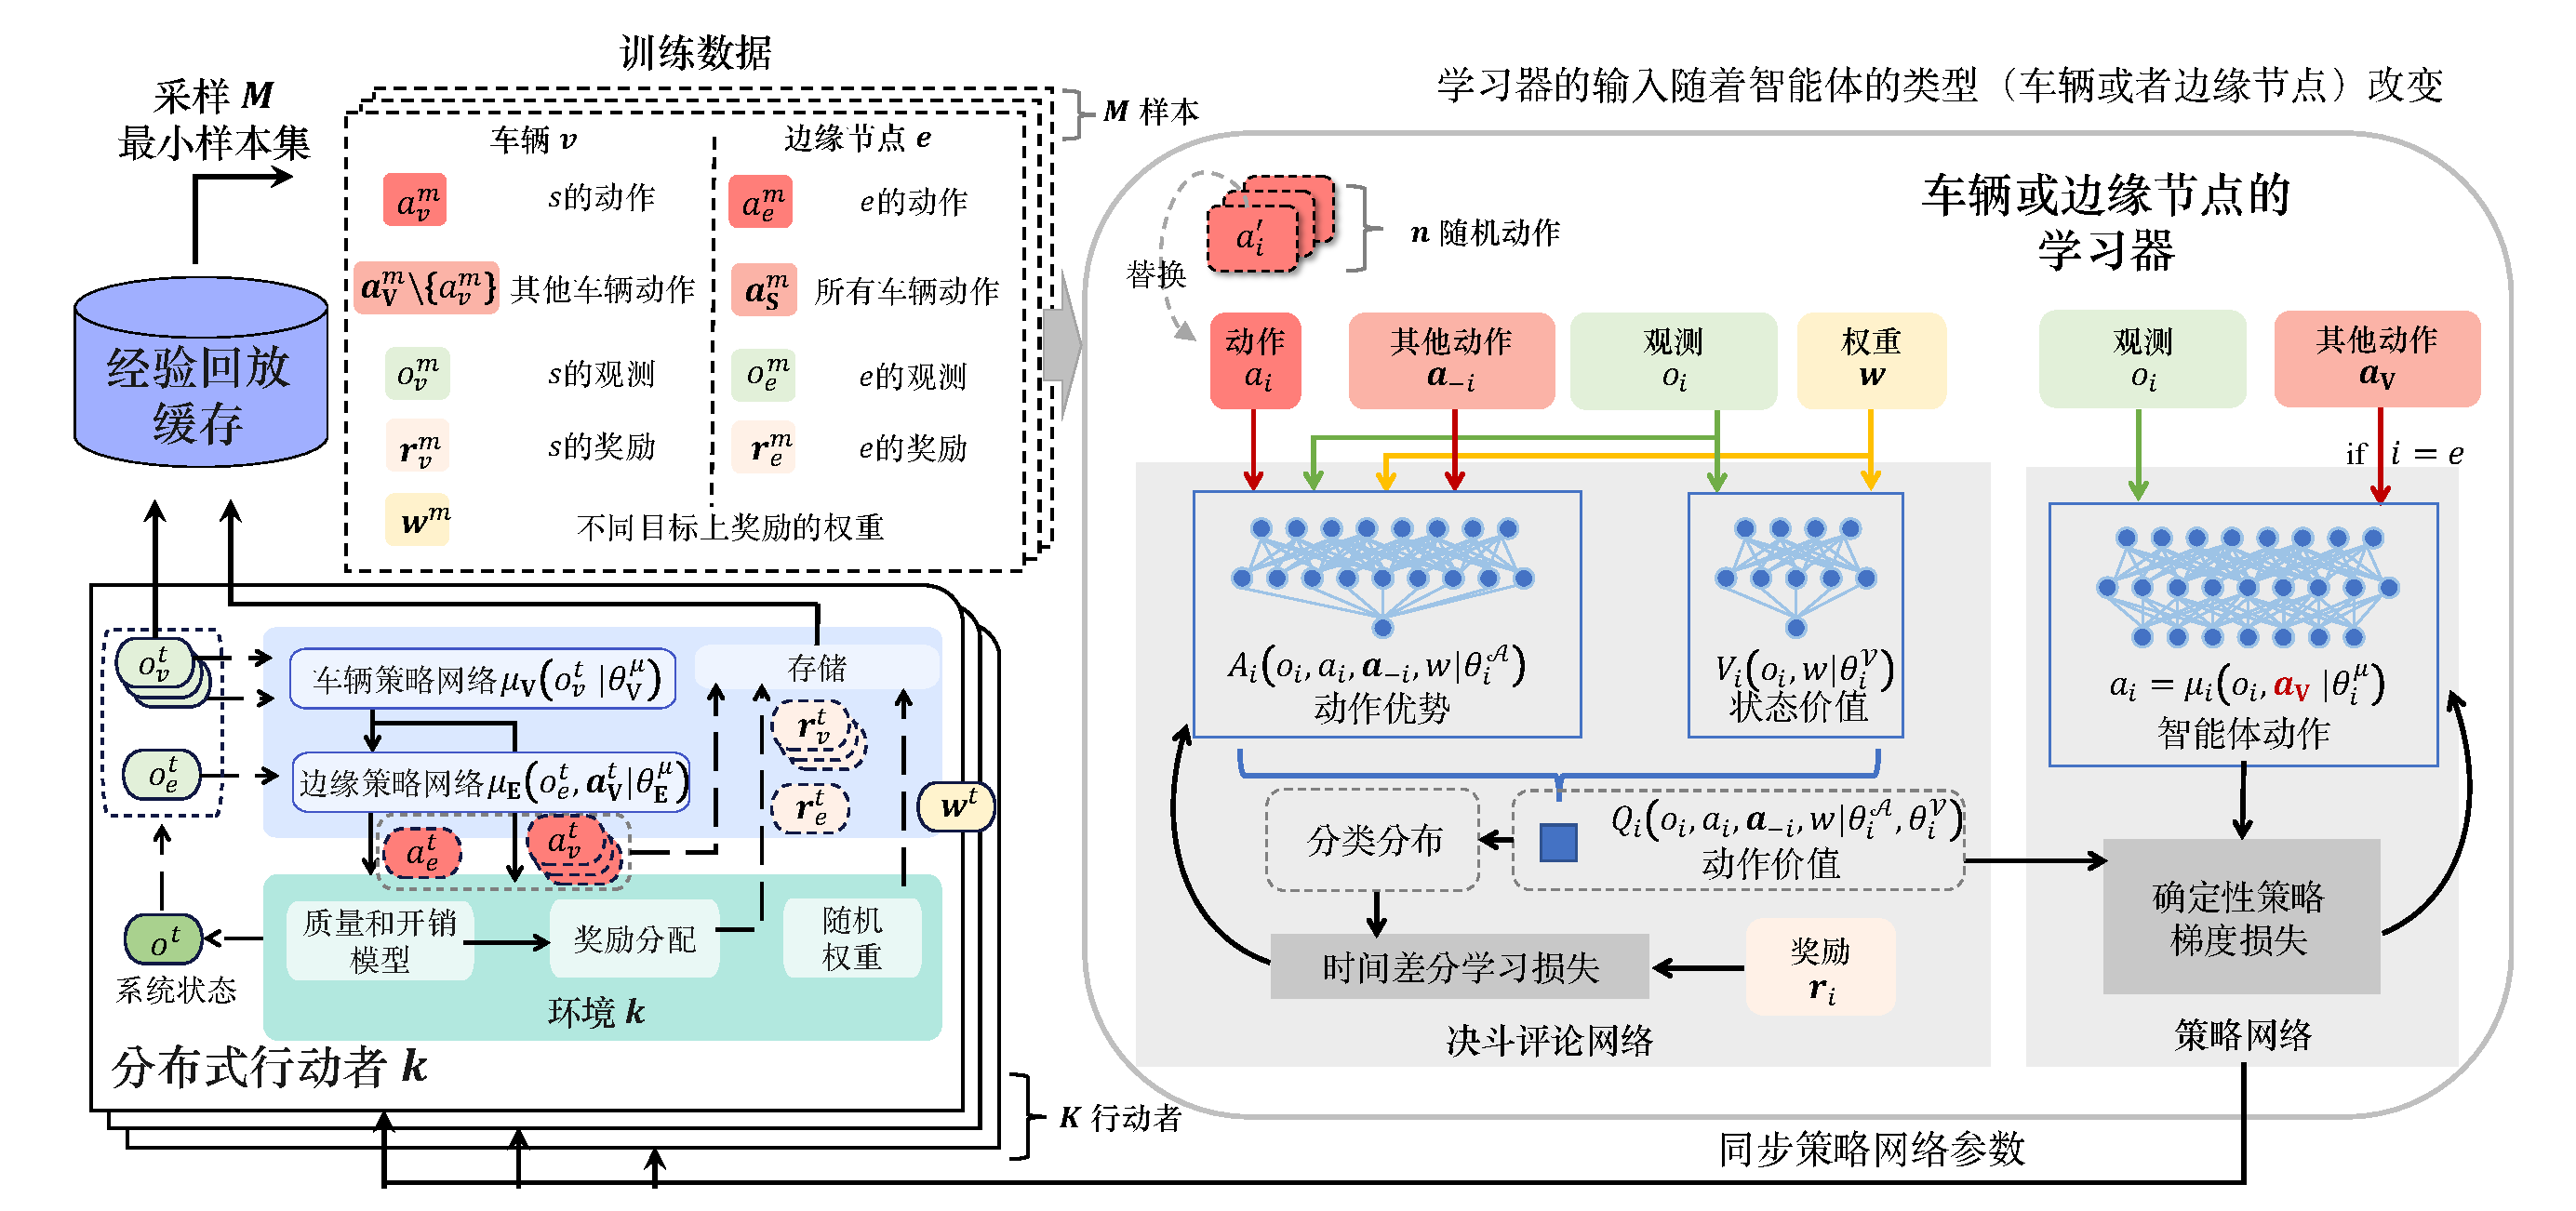
\includegraphics[width=0.65\textwidth]{fig/Fig4-2-solution-model.pdf}
\end{figure}
\end{textblock*}
\end{center}

\begin{center}
\begin{textblock*}{0.6\textwidth}(0.2cm,1.8cm)
\begin{itemize} \englishfont
	\item[\ding{111}] {\color{cqublue}{系统状态}}
	\item {\small{$\boldsymbol{o}_{v}^{t}=\left\{t, v, l_{v}^t, \mathbf{D}_{v}, \Phi_{v}, \mathbf{D}_{e}^{t}, \mathbf{D}_{\mathbf{I}_e^t}, \boldsymbol{w}^{t}\right\}$}}
	\item {\small{$\boldsymbol{o}_{e}^{t}=\left\{t, e, \operatorname{\mathbf{Dis}}_{\mathbf{V}, e}^{t}, \mathbf{D}_{1}, \ldots, \mathbf{D}_{V}, \mathbf{D}_{e}^{t}, \mathbf{D}_{\mathbf{I}_e^t}, \boldsymbol{w}^{t} \right\}$}}
	\item[\ding{111}] {\color{cqublue}{动作空间}}
	\item {\small{$\boldsymbol{a}_{v}^{t} = \{ \mathbf{C}_v^t,  \{ \lambda_{d, v}^{t}, p_{d, v}^{t} \mid \forall d \in \mathbf{D}_{v}^t \} , \pi_v^t   \}$}}
	\item {\small{$\boldsymbol{a}_{e}^{t} = \{b_{v, e}^{t} \mid \forall v \in \mathbf{V}_{e}^{t}\}$}}
	\item[\ding{111}] {\color{cqublue}{奖励函数}}
	\item {\small{$\boldsymbol{r}^{t} = \begin{bmatrix}  r^{(1)}\left(\boldsymbol{a}_{\mathbf{V}}^{t},\boldsymbol{a}_{e}^{t} \mid \boldsymbol{o}^{t}\right)  &  r^{(2)}\left(\boldsymbol{a}_{\mathbf{V}}^{t},\boldsymbol{a}_{e}^{t} \mid \boldsymbol{o}^{t}\right) \end{bmatrix} ^{T}$}}
	\item {\small{$r^{(1)}\left(\boldsymbol{a}_{\mathbf{V}}^{t},\boldsymbol{a}_{e}^{t} \mid \boldsymbol{o}^{t}\right)=\frac{1}{\left|\mathbf{I}_e^t\right|} \sum_{\forall i \in \mathbf{I}_e^t}\operatorname{QV}_{i}$}}
	\item {\small{$r^{(2)}\left(\boldsymbol{a}_{\mathbf{V}}^{t},\boldsymbol{a}_{e}^{t} \mid \boldsymbol{o}^{t}\right)=\frac{1}{\left|\mathbf{I}_e^t\right|} \sum_{\forall i \in \mathbf{I}_e^t} \operatorname{PV}_{j}$}}
\end{itemize}
\end{textblock*}
\end{center}
\end{frame}

\begin{frame}
\frametitle{\englishfont \underline{算法}:决斗评论家网络 (DCN)}
\newBackground
\begin{center}
\begin{textblock*}{\textwidth}(4.5cm,2.6cm)
\begin{figure}
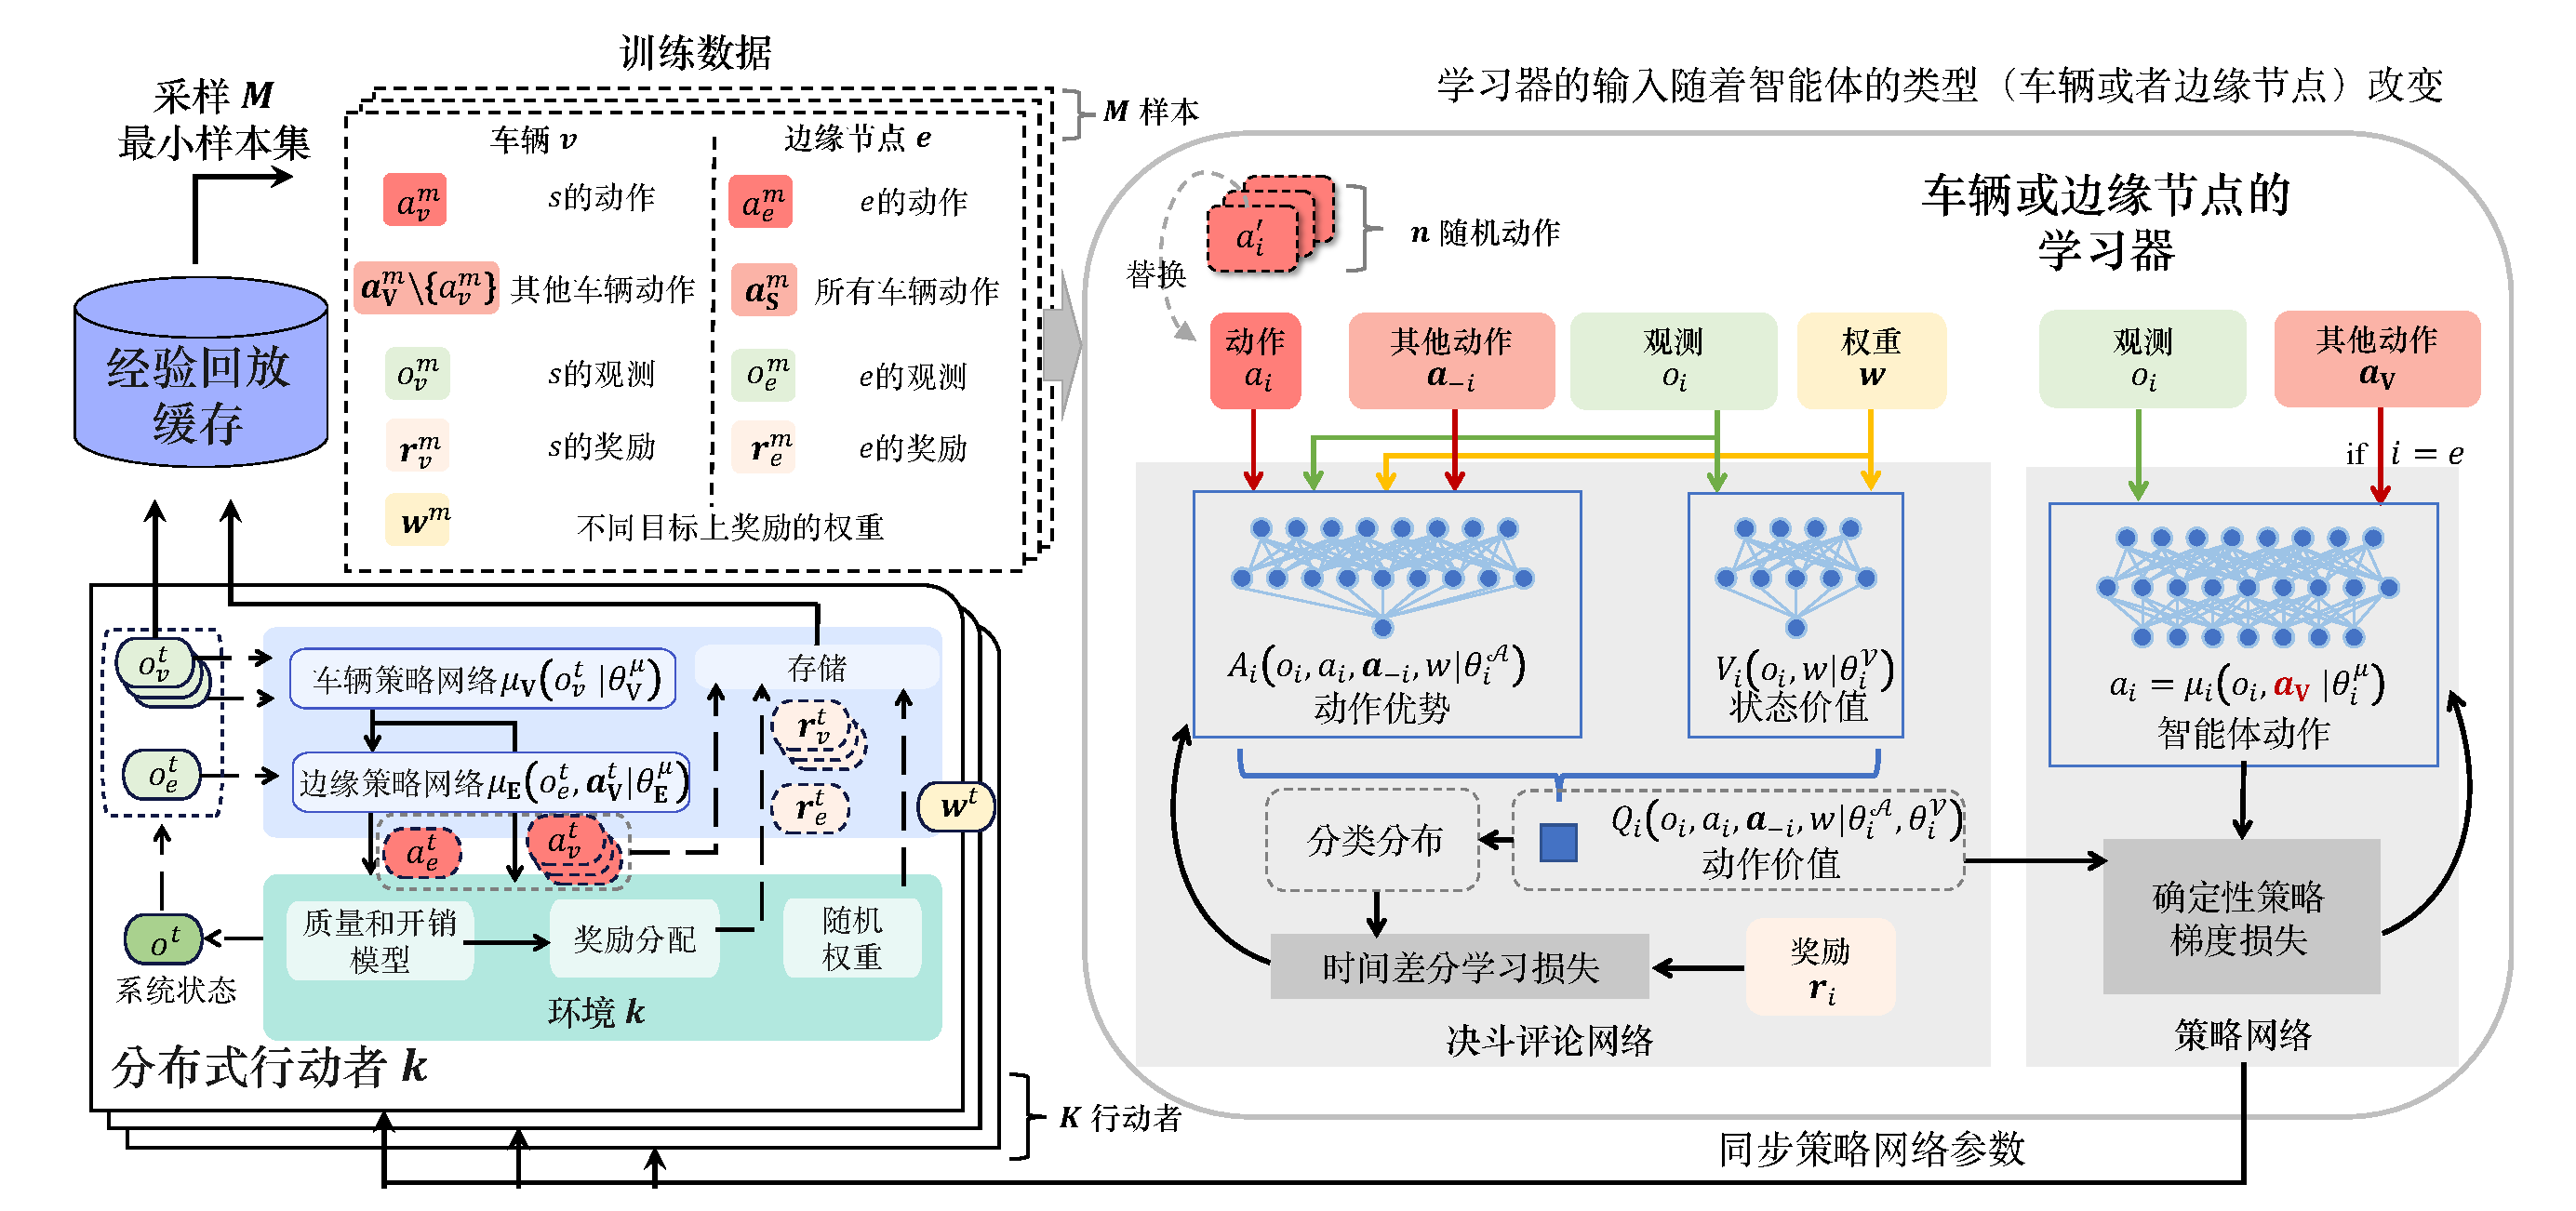
\includegraphics[width=0.65\textwidth]{fig/Fig4-2-solution-model.pdf}
\end{figure}
\end{textblock*}
\end{center}

\begin{center}
\begin{textblock*}{0.6\textwidth}(0.2cm,5.5cm)
\begin{align} \footnotesize
    & Q_{\mathbf{V}}\left({o}_{v}^{m}, {a}_{v}^{m}, \boldsymbol{a}_{\boldsymbol{\mathbf{V}}-v}^{m}, \boldsymbol{w}^{m} \mid \theta_{\mathbf{V}}^{Q} \right) \notag \\
    &= V_{\mathbf{V}}\left({o}_{v}^{m}, \boldsymbol{w}^{m} \mid \theta_{\mathbf{V}}^{\mathscr{V}} \right) + A_{\mathbf{V}}\left({o}_{v}^{m},  {a}_{v}^{m}, \boldsymbol{a}_{\boldsymbol{\mathbf{V}}-v}^{m}, \boldsymbol{w}^{m} \mid \theta_{\mathbf{V}}^{\mathscr{A}} \right) \notag \\
    &- \frac{1}{N} \sum_{\forall n} A_{\mathbf{V}}\left({o}_{v}^{m},  {a}_{v}^{m, n}, \boldsymbol{a}_{\boldsymbol{\mathbf{V}}-v}^{m}, \boldsymbol{w}^{m} \mid \theta_{\mathbf{V}}^{\mathscr{A}} \right) \notag
\end{align}

\end{textblock*}
\end{center}

\begin{center}
\begin{textblock*}{0.6\textwidth}(0.2cm,1.8cm)
\begin{itemize} \englishfont
	\item[\ding{111}] {\color{cqublue}{动作优势网络 (AA)}}
	\item 车辆 {\small{$A_{\mathbf{V}}\left({o}_{v}^{m},  {a}_{v}^{m}, \boldsymbol{a}_{\boldsymbol{\mathbf{V}}-v}^{m}, \boldsymbol{w}^{m} \mid \theta_{\mathbf{V}}^{\mathscr{A}} \right)$}}
	\item 边缘节点 {\small{$A_{\mathbf{E}}\left({o}_{e}^{m},  {a}_{e}^{m}, \boldsymbol{a}_{\boldsymbol{\mathbf{V}}}^{m}, \boldsymbol{w}^{m} \mid \theta_{\mathbf{E}}^{\mathscr{A}} \right)$}}
	\item[\ding{111}] {\color{cqublue}{状态价值网络 (SV)}}
	\item 车辆 {\small{$V_{\mathbf{V}}\left({o}_{v}^{m}, \boldsymbol{w}^{m} \mid \theta_{\mathbf{V}}^{\mathscr{V}} \right)$}}
	\item 边缘节点 {\small{$V_{\mathbf{E}}\left({o}_{e}^{m}, \boldsymbol{w}^{m} \mid \theta_{\mathbf{E}}^{\mathscr{V}} \right)$}}
	\item[\ding{111}] {\color{cqublue}{动作价值}}
	\item 
\end{itemize}
\end{textblock*}
\end{center}
\end{frame}

\begin{frame}
\frametitle{\englishfont \underline{实验}:数据与基本设置}
\newBackground

\begin{center}
	\begin{textblock*}{\textwidth}(-3.2cm,2.3cm)
	\begin{table}[h] \englishfont
\resizebox{0.5\textwidth}{!}{%
\begin{tabular}{cc}
\toprule 
\textbf{参数} & \textbf{值}         \\ \midrule
最大传输功率        & 100 mW               \\
传输可靠性阈值       & 0.9           \\
及时性加权系数          & 0.6              \\
一致性加权系数 & 0.4\\
冗余度加权系数 & 0.2 \\
感知开销加权系数         & 0.4  \\
传输开销加权系数         & 0.4  \\
策略网络        & 4 层全连接 (隐藏层 256-128)  \\
评论家网络         & 4 层全连接 (隐藏层 512-256) \\
学习率         & 1$\times10^{-4}$              \\
折扣因子        & 0.996              \\
经验回放缓存大小    & 1$\times10^{6}$          \\
批大小         & 256                \\ \bottomrule
\end{tabular}%
}
\end{table}
\end{textblock*}
\end{center}

\begin{center}
\begin{textblock*}{\textwidth}(0cm,1.8cm)
\begin{itemize} \englishfont
	\item[\ding{111}] {\color{cqublue}{实验与模型参数}}
\end{itemize}
\end{textblock*}
\end{center}

\begin{center}
\begin{textblock*}{0.65\textwidth}(7cm,1.8cm)
\begin{itemize}[itemsep=0.2\baselineskip]  \englishfont 
	\item[\ding{111}] {\color{cqublue}{对比算法}}
	\begin{itemize}[itemsep=0.2\baselineskip] 
	\begin{small}
		\item[\ding{226}] 随机分配 ({\color{red}{RA}})
		\item[\ding{226}] 分布式深度确定性策略梯度 ({\color{red}{D4PG}})
		\item[\ding{226}] 多智能体分布式深度确定性策略梯度 ({\color{red}{MAD4PG}})
		\item
	\end{small}
	\end{itemize}
\end{itemize}
\end{textblock*}
\end{center}

\begin{center}
\begin{textblock*}{0.65\textwidth}(7cm,3.85cm)
\begin{itemize}[itemsep=0.2\baselineskip] \englishfont
	\item[\ding{111}] {\color{cqublue}{性能评估指标}}
	\begin{itemize}[itemsep=0.2\baselineskip]
	\begin{small}
		\item[\ding{226}] 单位开销质量 ({\color{red}{QPUC}})\\
		{\small{$\operatorname{QPUC}=\frac{\sum_{\forall t \in \mathbf{T}} \sum_{\forall e \in \mathbf{E}} \sum_{\forall i \in \mathbf{I}_e^t} \mathrm{QV}_i}{\sum_{\forall t \in \mathbf{T}} \sum_{\forall e \in \mathbf{E}} \sum_{\forall i \in \mathbf{I}_e^t} \mathrm{CV}_i}$}}
		\item[\ding{226}] 单位质量利润 ({\color{red}{PPUQ}})\\
		{\small{$\operatorname{PPUQ}=\frac{\sum_{\forall t \in \mathbf{T}} \sum_{\forall e \in \mathbf{E}} \sum_{\forall i \in \mathbf{I}_e^t}\mathrm{PV}_i}{\sum_{\forall t \in \mathbf{T}} \sum_{\forall e \in \mathbf{E}} \sum_{\forall i \in \mathbf{I}_e^t} \mathrm{QV}_i}$}}
		\item[\ding{226}] 平均及时性 ({\color{red}{AT}}) \hspace{1em}平均冗余度 ({\color{red}{AR}})
		\item [\ding{226}] 平均感知开销({\color{red}{ASC}}) \hspace{1em}平均传输开销({\color{red}{ATC}})
	\end{small}
	\end{itemize}
\end{itemize}
\end{textblock*}
\end{center}

\end{frame}

\begin{frame}
\newBackground

\begin{overlayarea}{\textwidth}{3cm}
\only<1-1>{
\frametitle{\englishfont \underline{实验}:算法收敛性}
\begin{center} \englishfont \footnotesize
\begin{textblock*}{\textwidth}(1cm,2.2cm)
	\begin{figure}
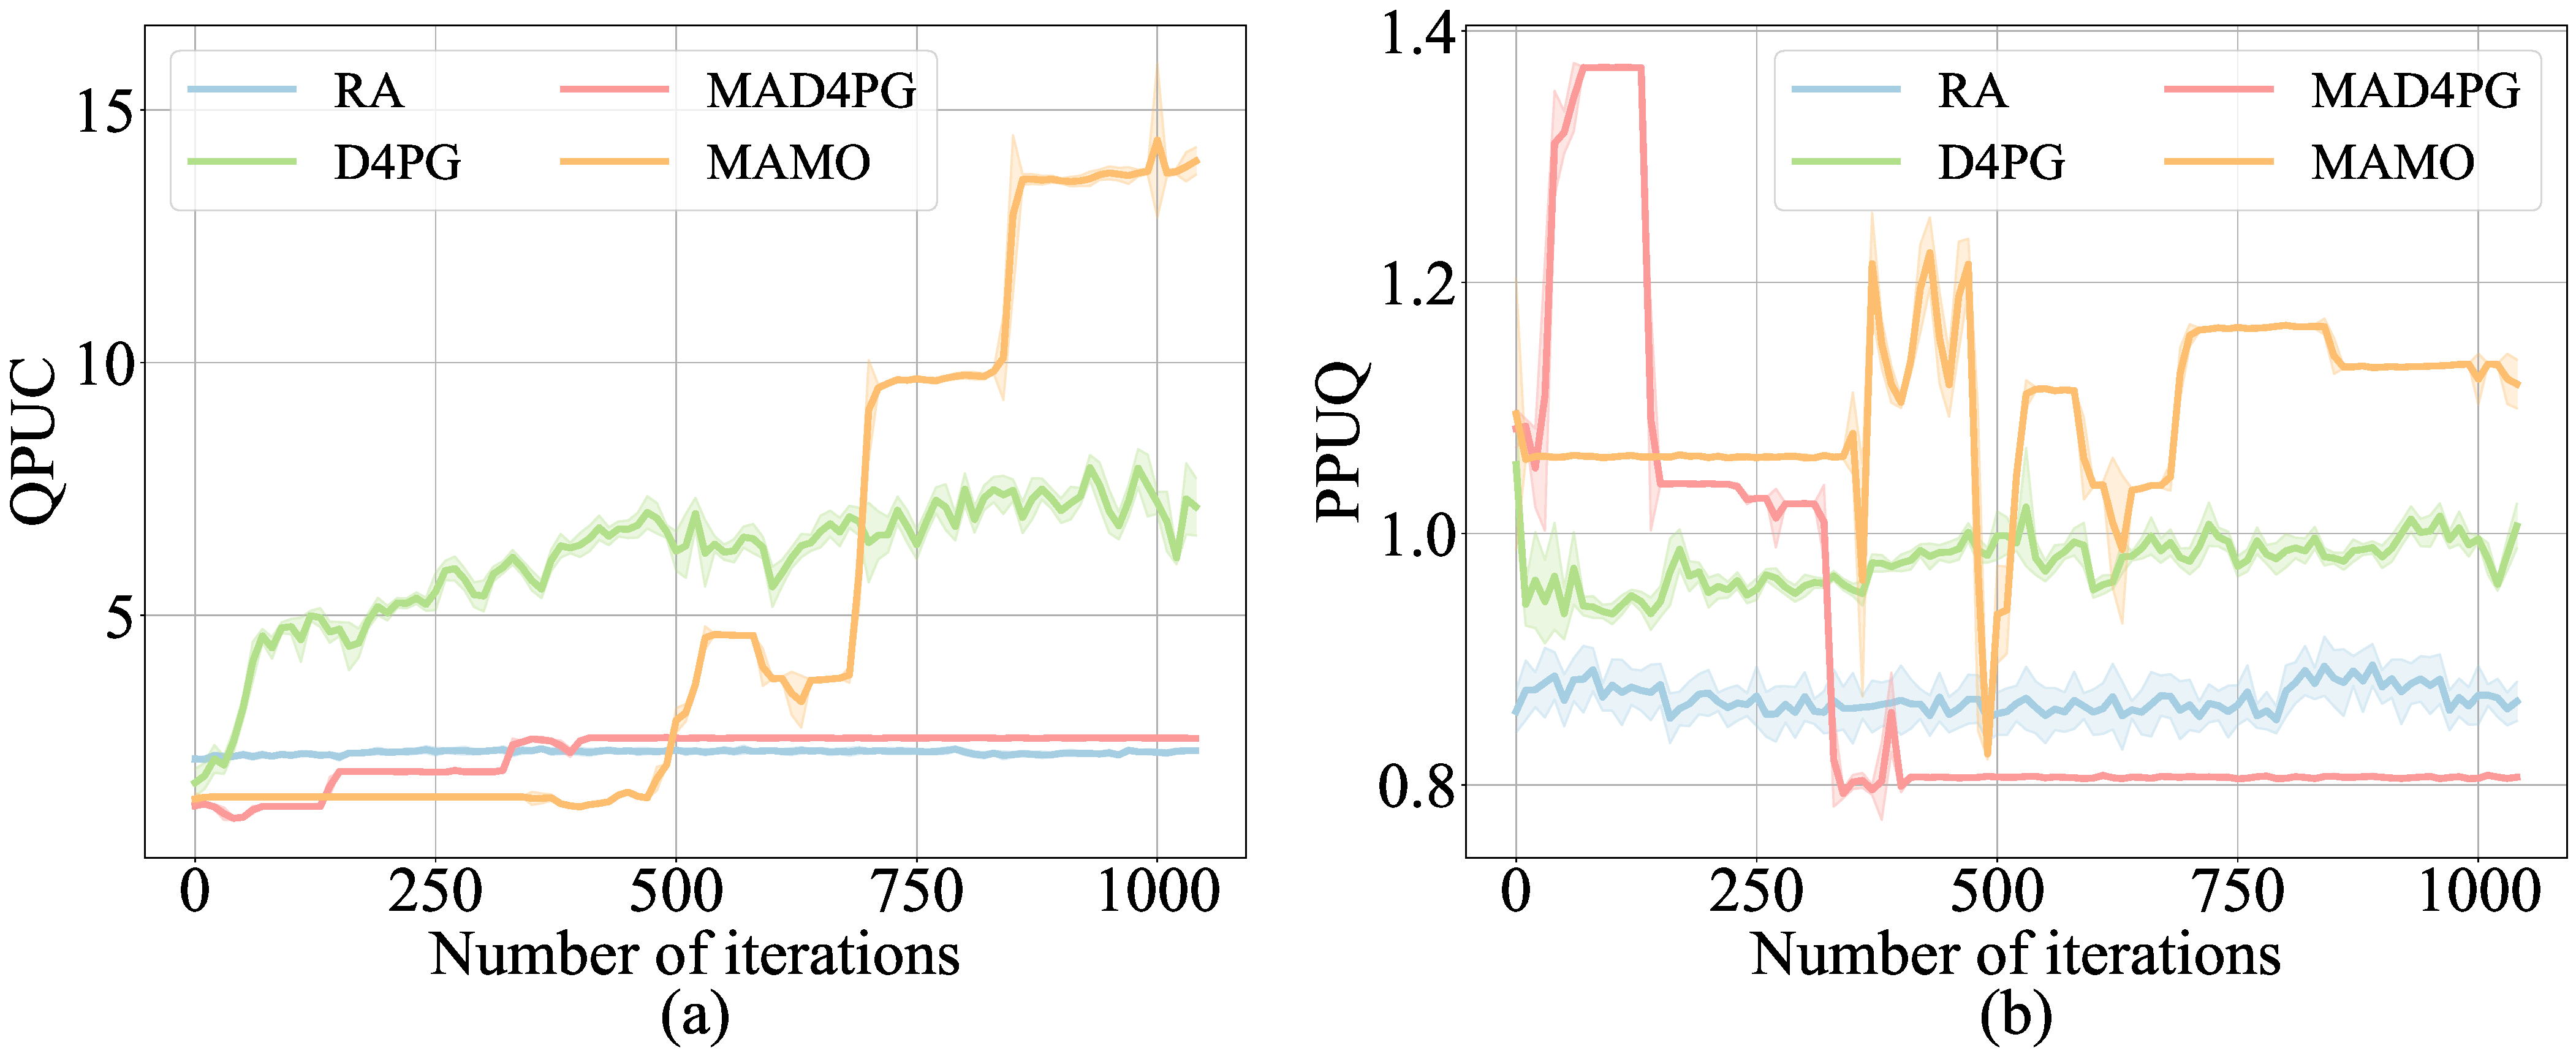
\includegraphics[width=1\textwidth]{fig/Fig4-3-different-algorithms.pdf}
	\end{figure}
\end{textblock*}
\end{center}
}

\only<2-2>{
\frametitle{\englishfont \underline{实验}:算法收敛性}
\begin{center} \englishfont \footnotesize
\begin{textblock*}{\textwidth}(1cm,2.2cm)
	\begin{figure}
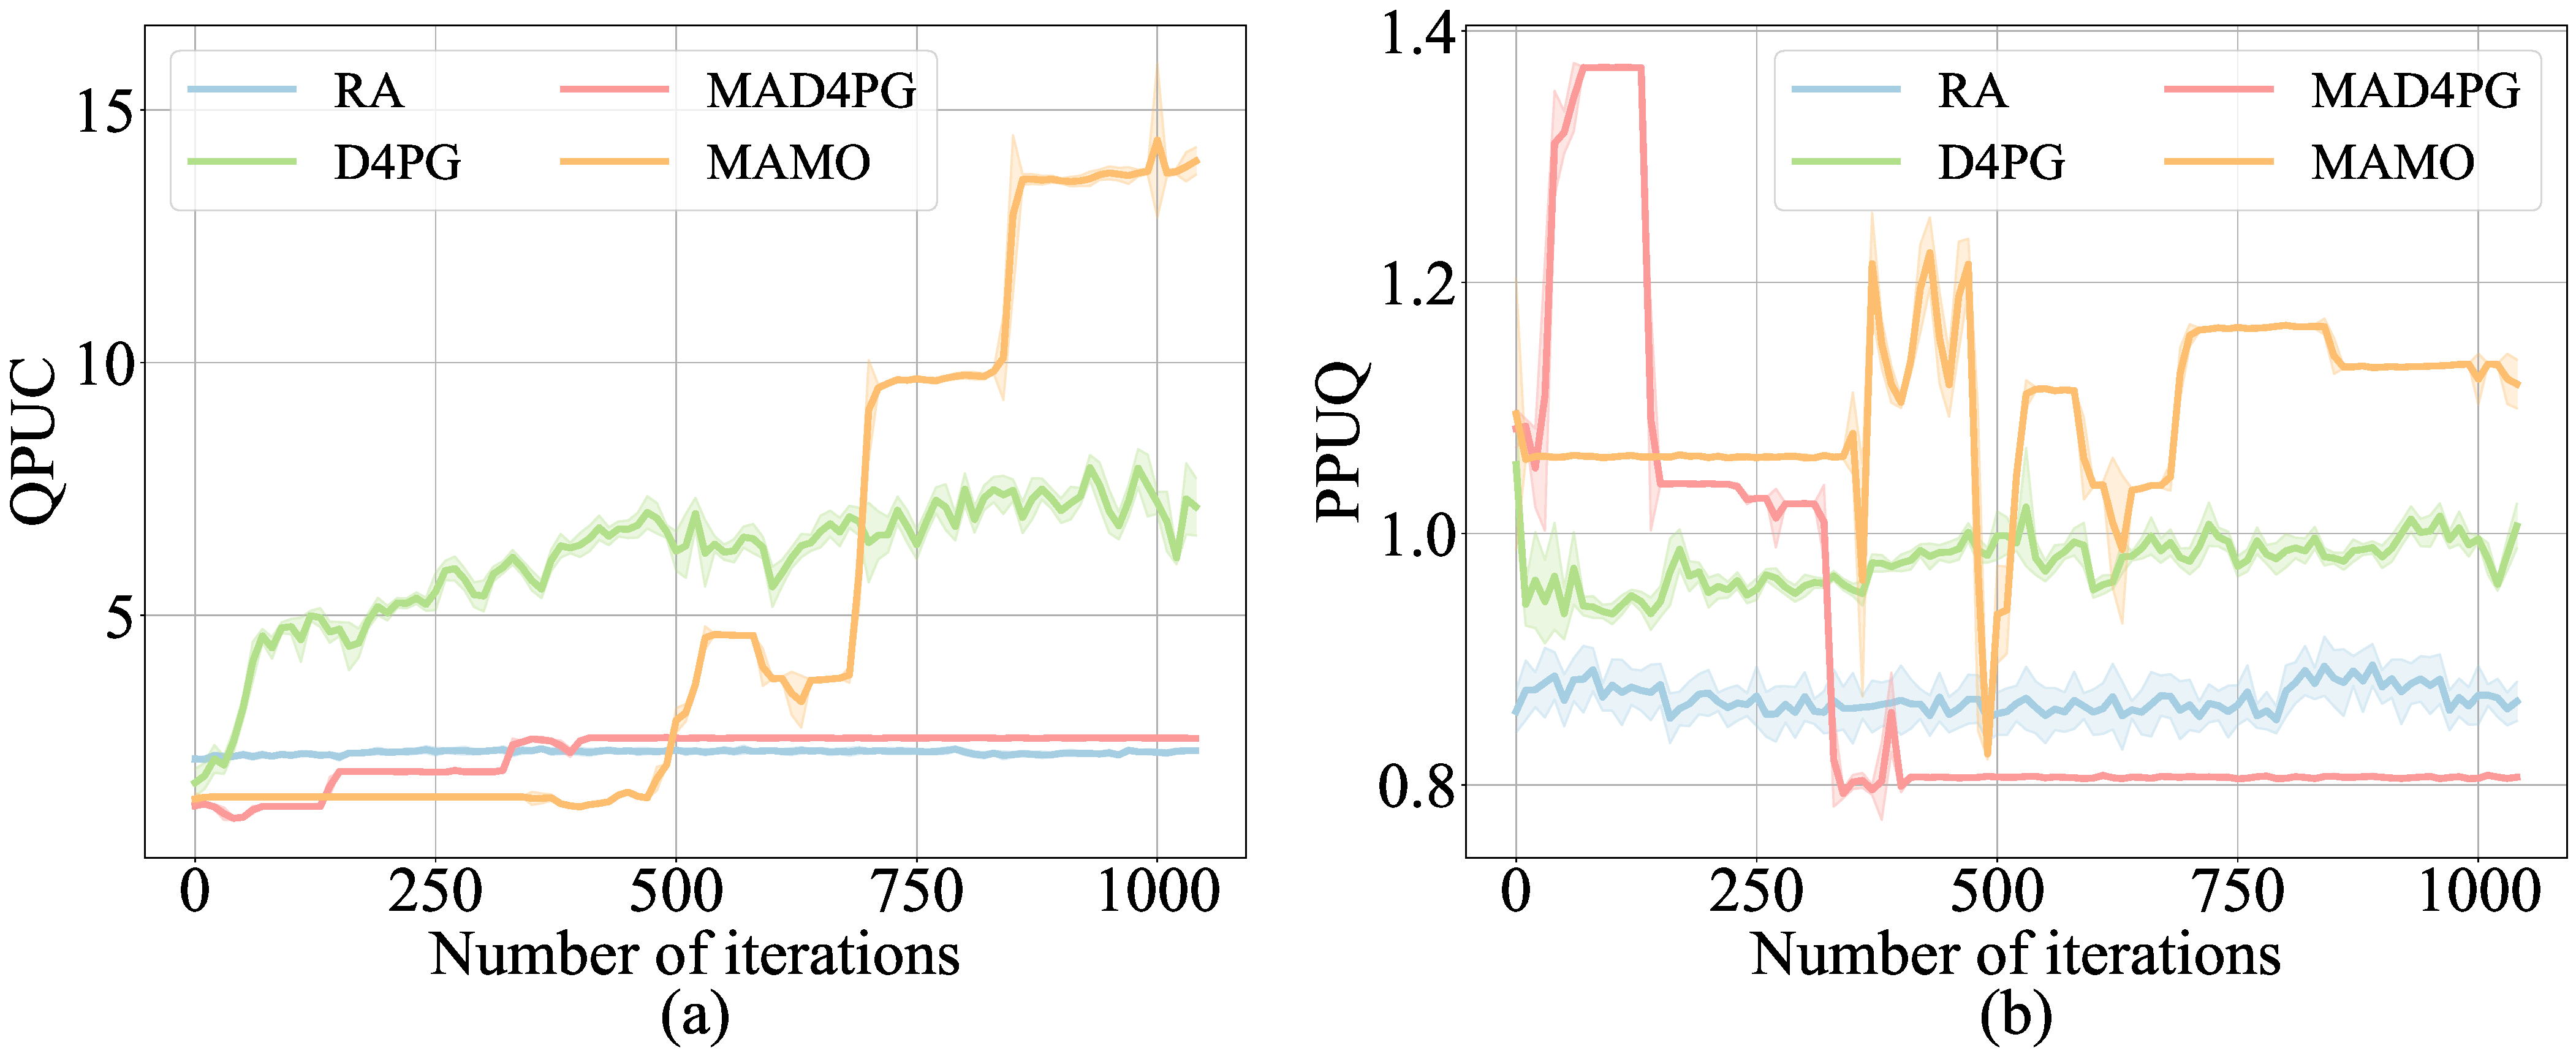
\includegraphics[width=1\textwidth]{fig/Fig4-3-different-algorithms.pdf}
	\end{figure}
\end{textblock*}
\end{center}
}

\only<2-2>{
\begin{center} \englishfont \footnotesize
\begin{textblock*}{\textwidth}(0cm,2.55cm)
{\Huge{\color{red}\ding{216}}}
\end{textblock*}
\end{center}

\begin{center} \englishfont \footnotesize
\begin{textblock*}{\textwidth}(6.95cm,3.5cm)
{\Huge{\color{red}\ding{216}}}
\end{textblock*}
\end{center}
}

\only<3-3>{
\frametitle{\englishfont \underline{实验}:神经元数量的影响}
\begin{center} \englishfont \footnotesize
\begin{textblock*}{\textwidth}(1cm,2.2cm)
	\begin{figure}
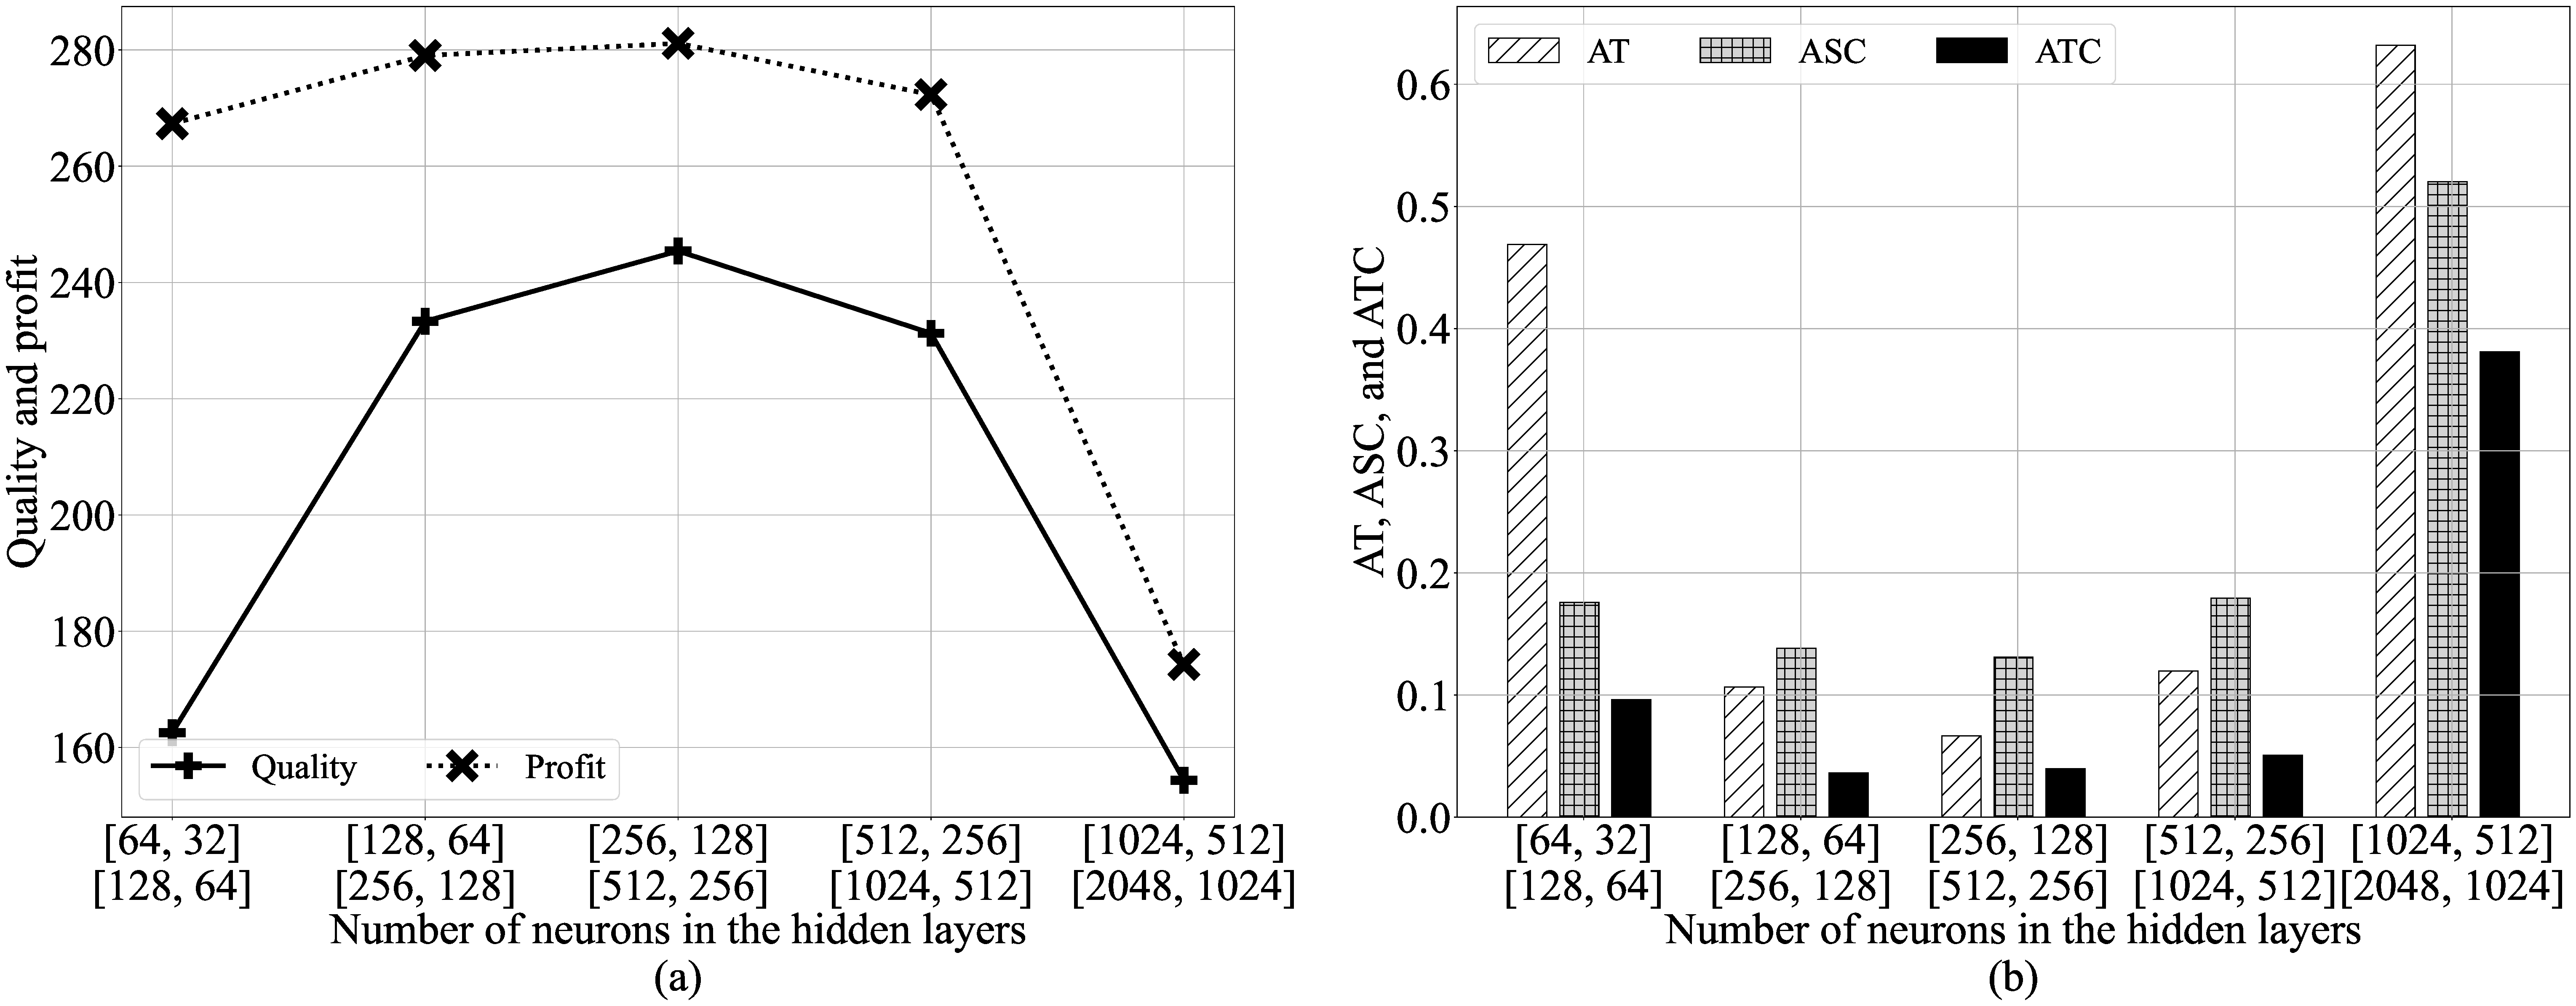
\includegraphics[width=1\textwidth]{fig/Fig4-4-different-networks.pdf}
	\end{figure}
\end{textblock*}
\end{center}
}

\only<4-4>{
\frametitle{\englishfont \underline{实验}:神经元数量的影响}
\begin{center} \englishfont \footnotesize
\begin{textblock*}{\textwidth}(1cm,2.2cm)
	\begin{figure}
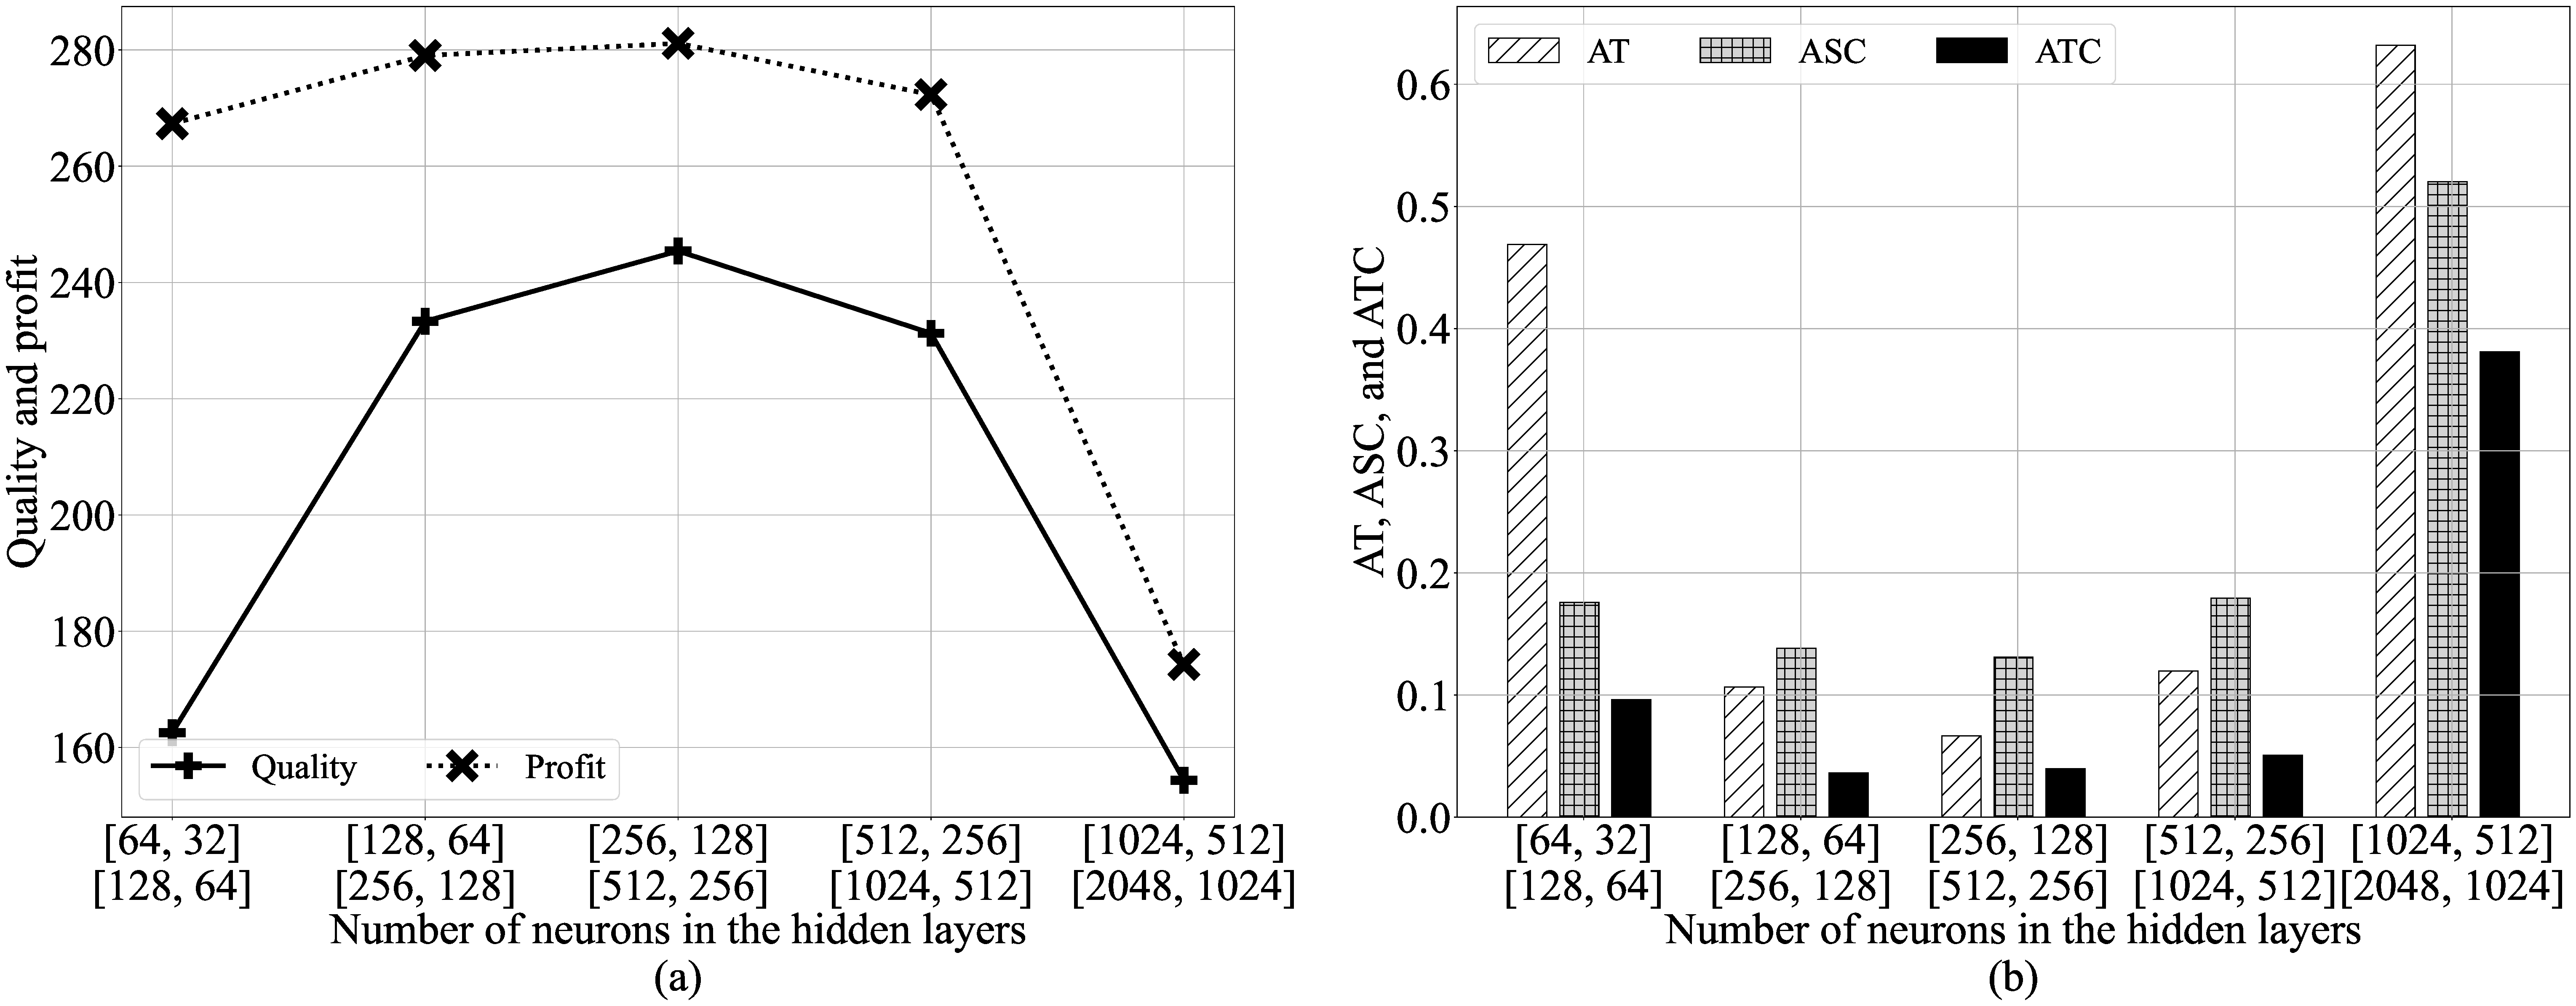
\includegraphics[width=1\textwidth]{fig/Fig4-4-different-networks.pdf}
	\end{figure}
\end{textblock*}
\end{center}
}

\only<4-4>{
\begin{center} \englishfont \footnotesize
\begin{textblock*}{\textwidth}(-2.45cm,1.9cm)
{\Huge{\color{red}\ding{216}}}
\end{textblock*}
\end{center}

\begin{center} \englishfont \footnotesize
\begin{textblock*}{\textwidth}(4.7cm,5.3cm)
{\Huge{\color{red}\ding{216}}}
\end{textblock*}
\end{center}

}

\only<5-5>{
\frametitle{\englishfont \underline{实验}:交通场景的影响}
\begin{center} \englishfont \footnotesize
\begin{textblock*}{\textwidth}(1cm,1.8cm)
	\begin{figure}
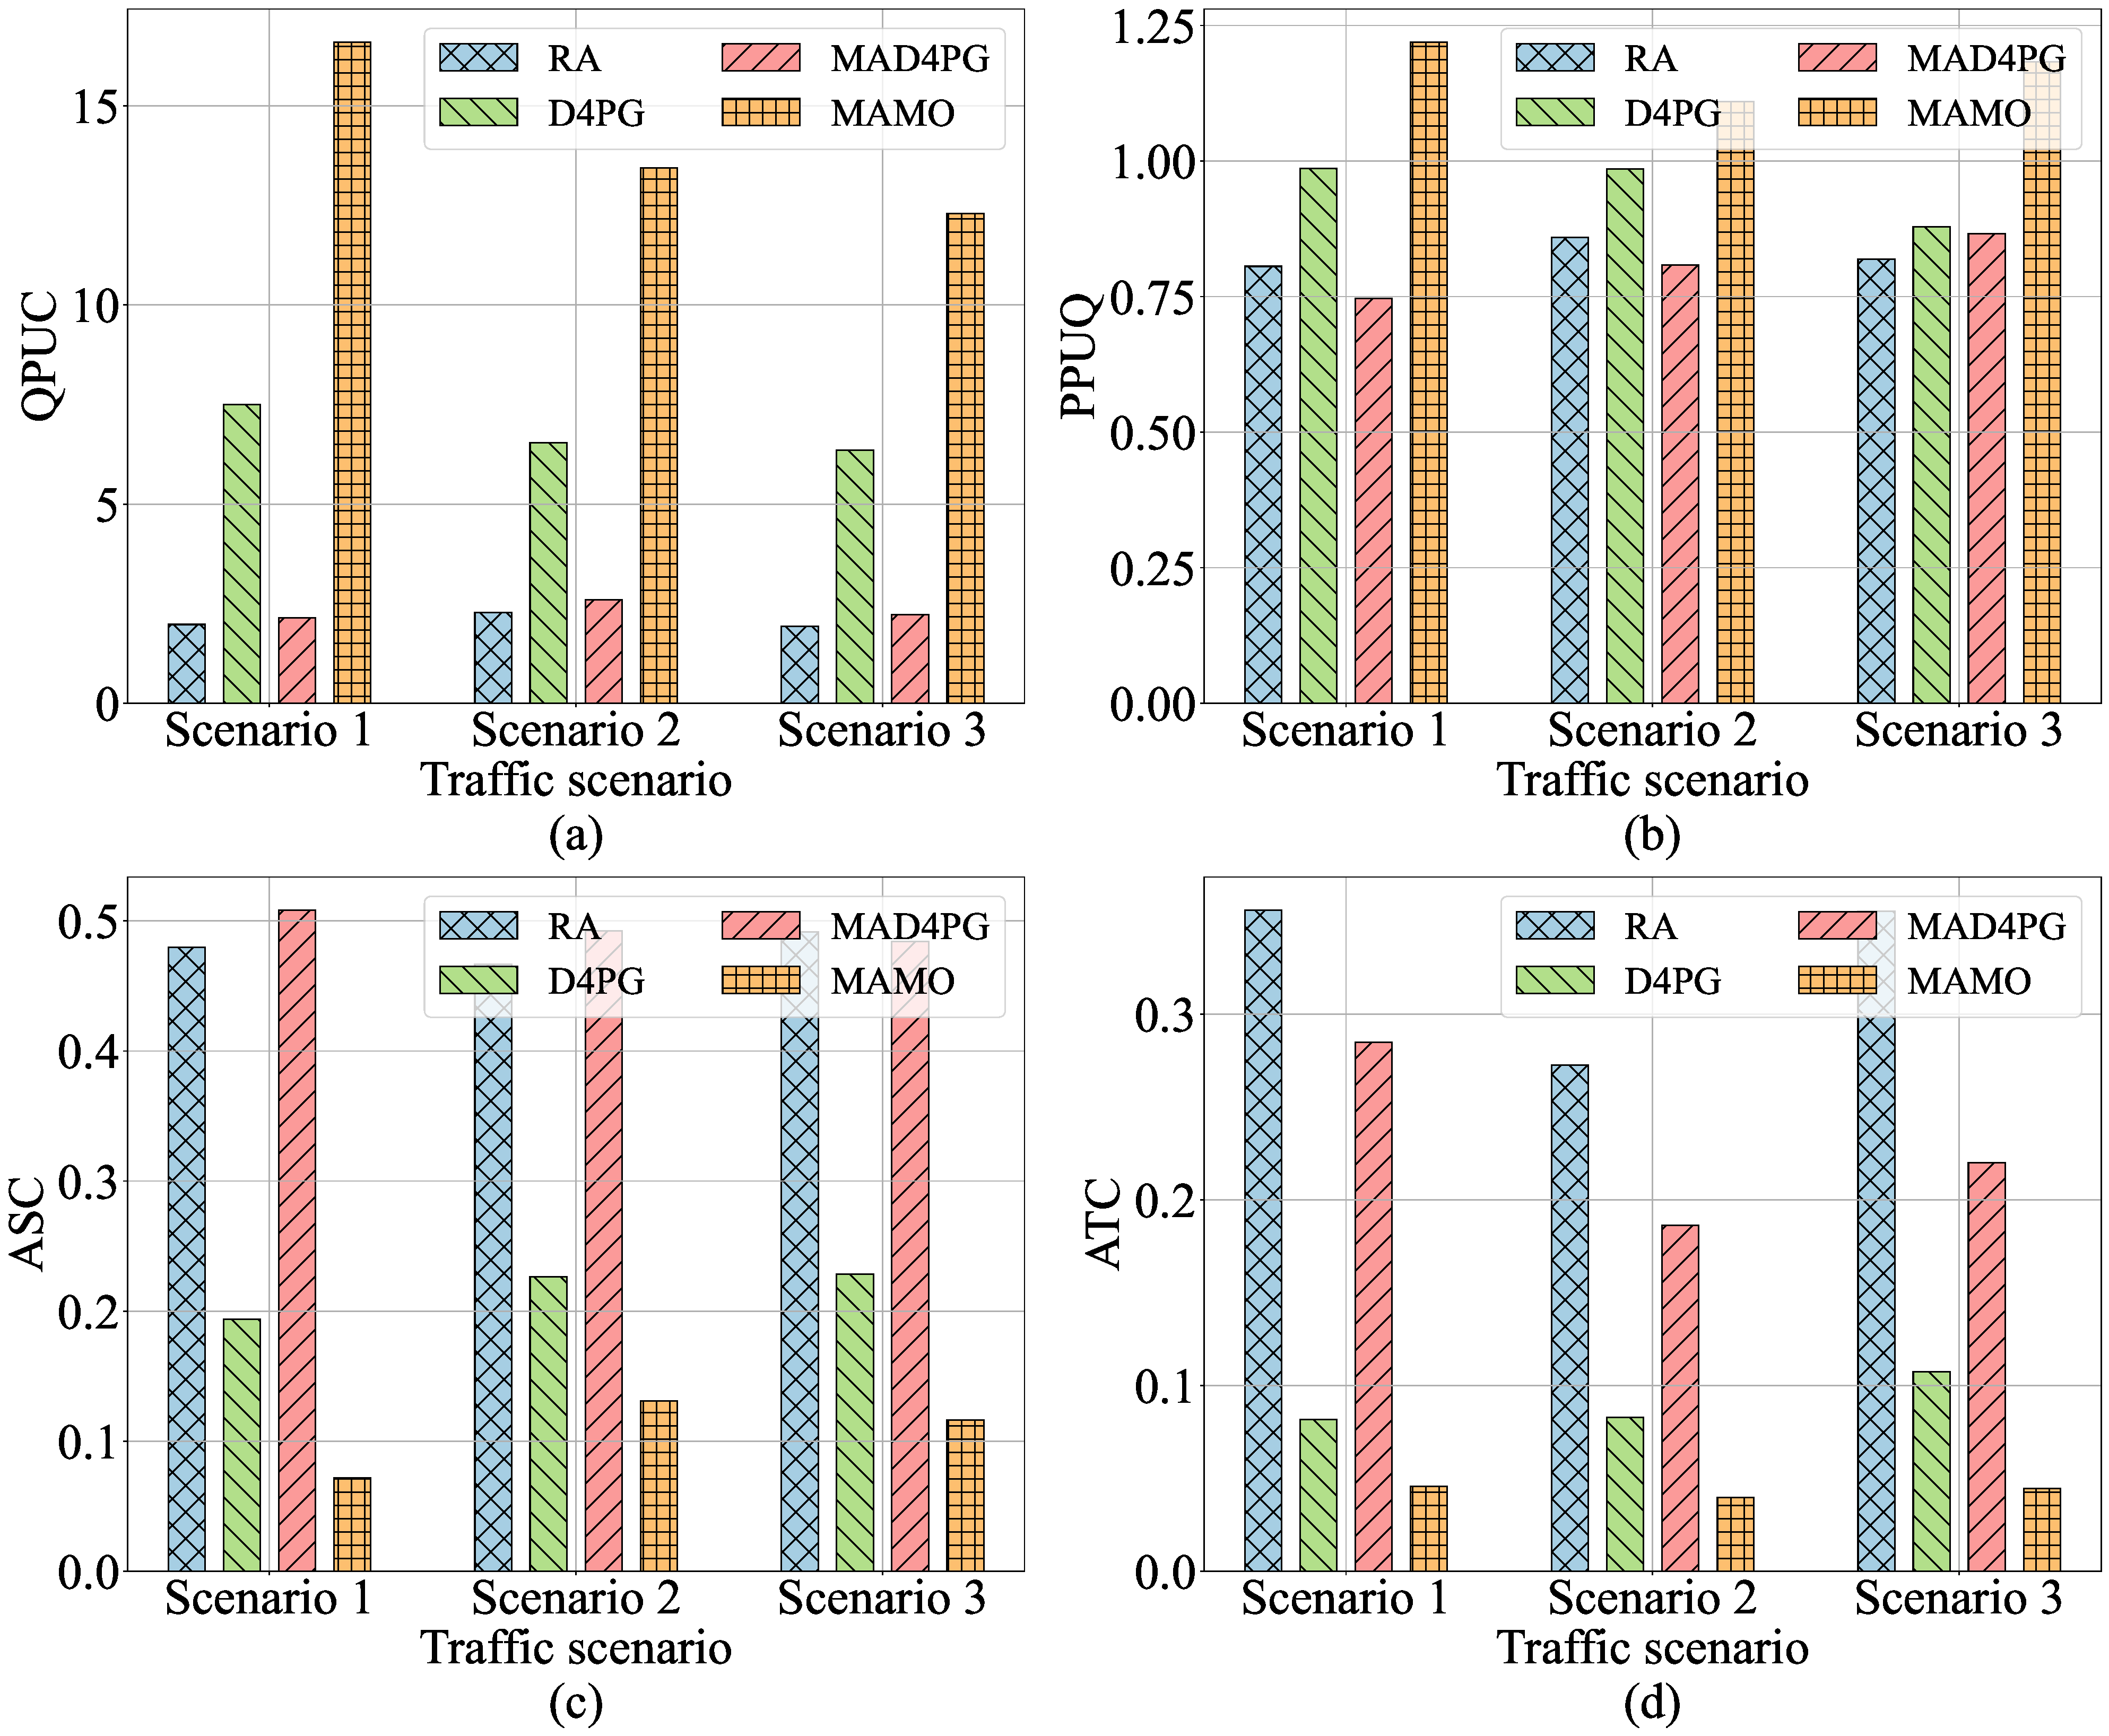
\includegraphics[width=0.55\textwidth]{fig/Fig4-5-different-scenarios.pdf}
	\end{figure}
\end{textblock*}
\end{center}
}

\only<6-6>{
\frametitle{\englishfont \underline{实验}:交通场景的影响}
\begin{center} \englishfont \footnotesize
\begin{textblock*}{\textwidth}(1cm,1.8cm)
	\begin{figure}
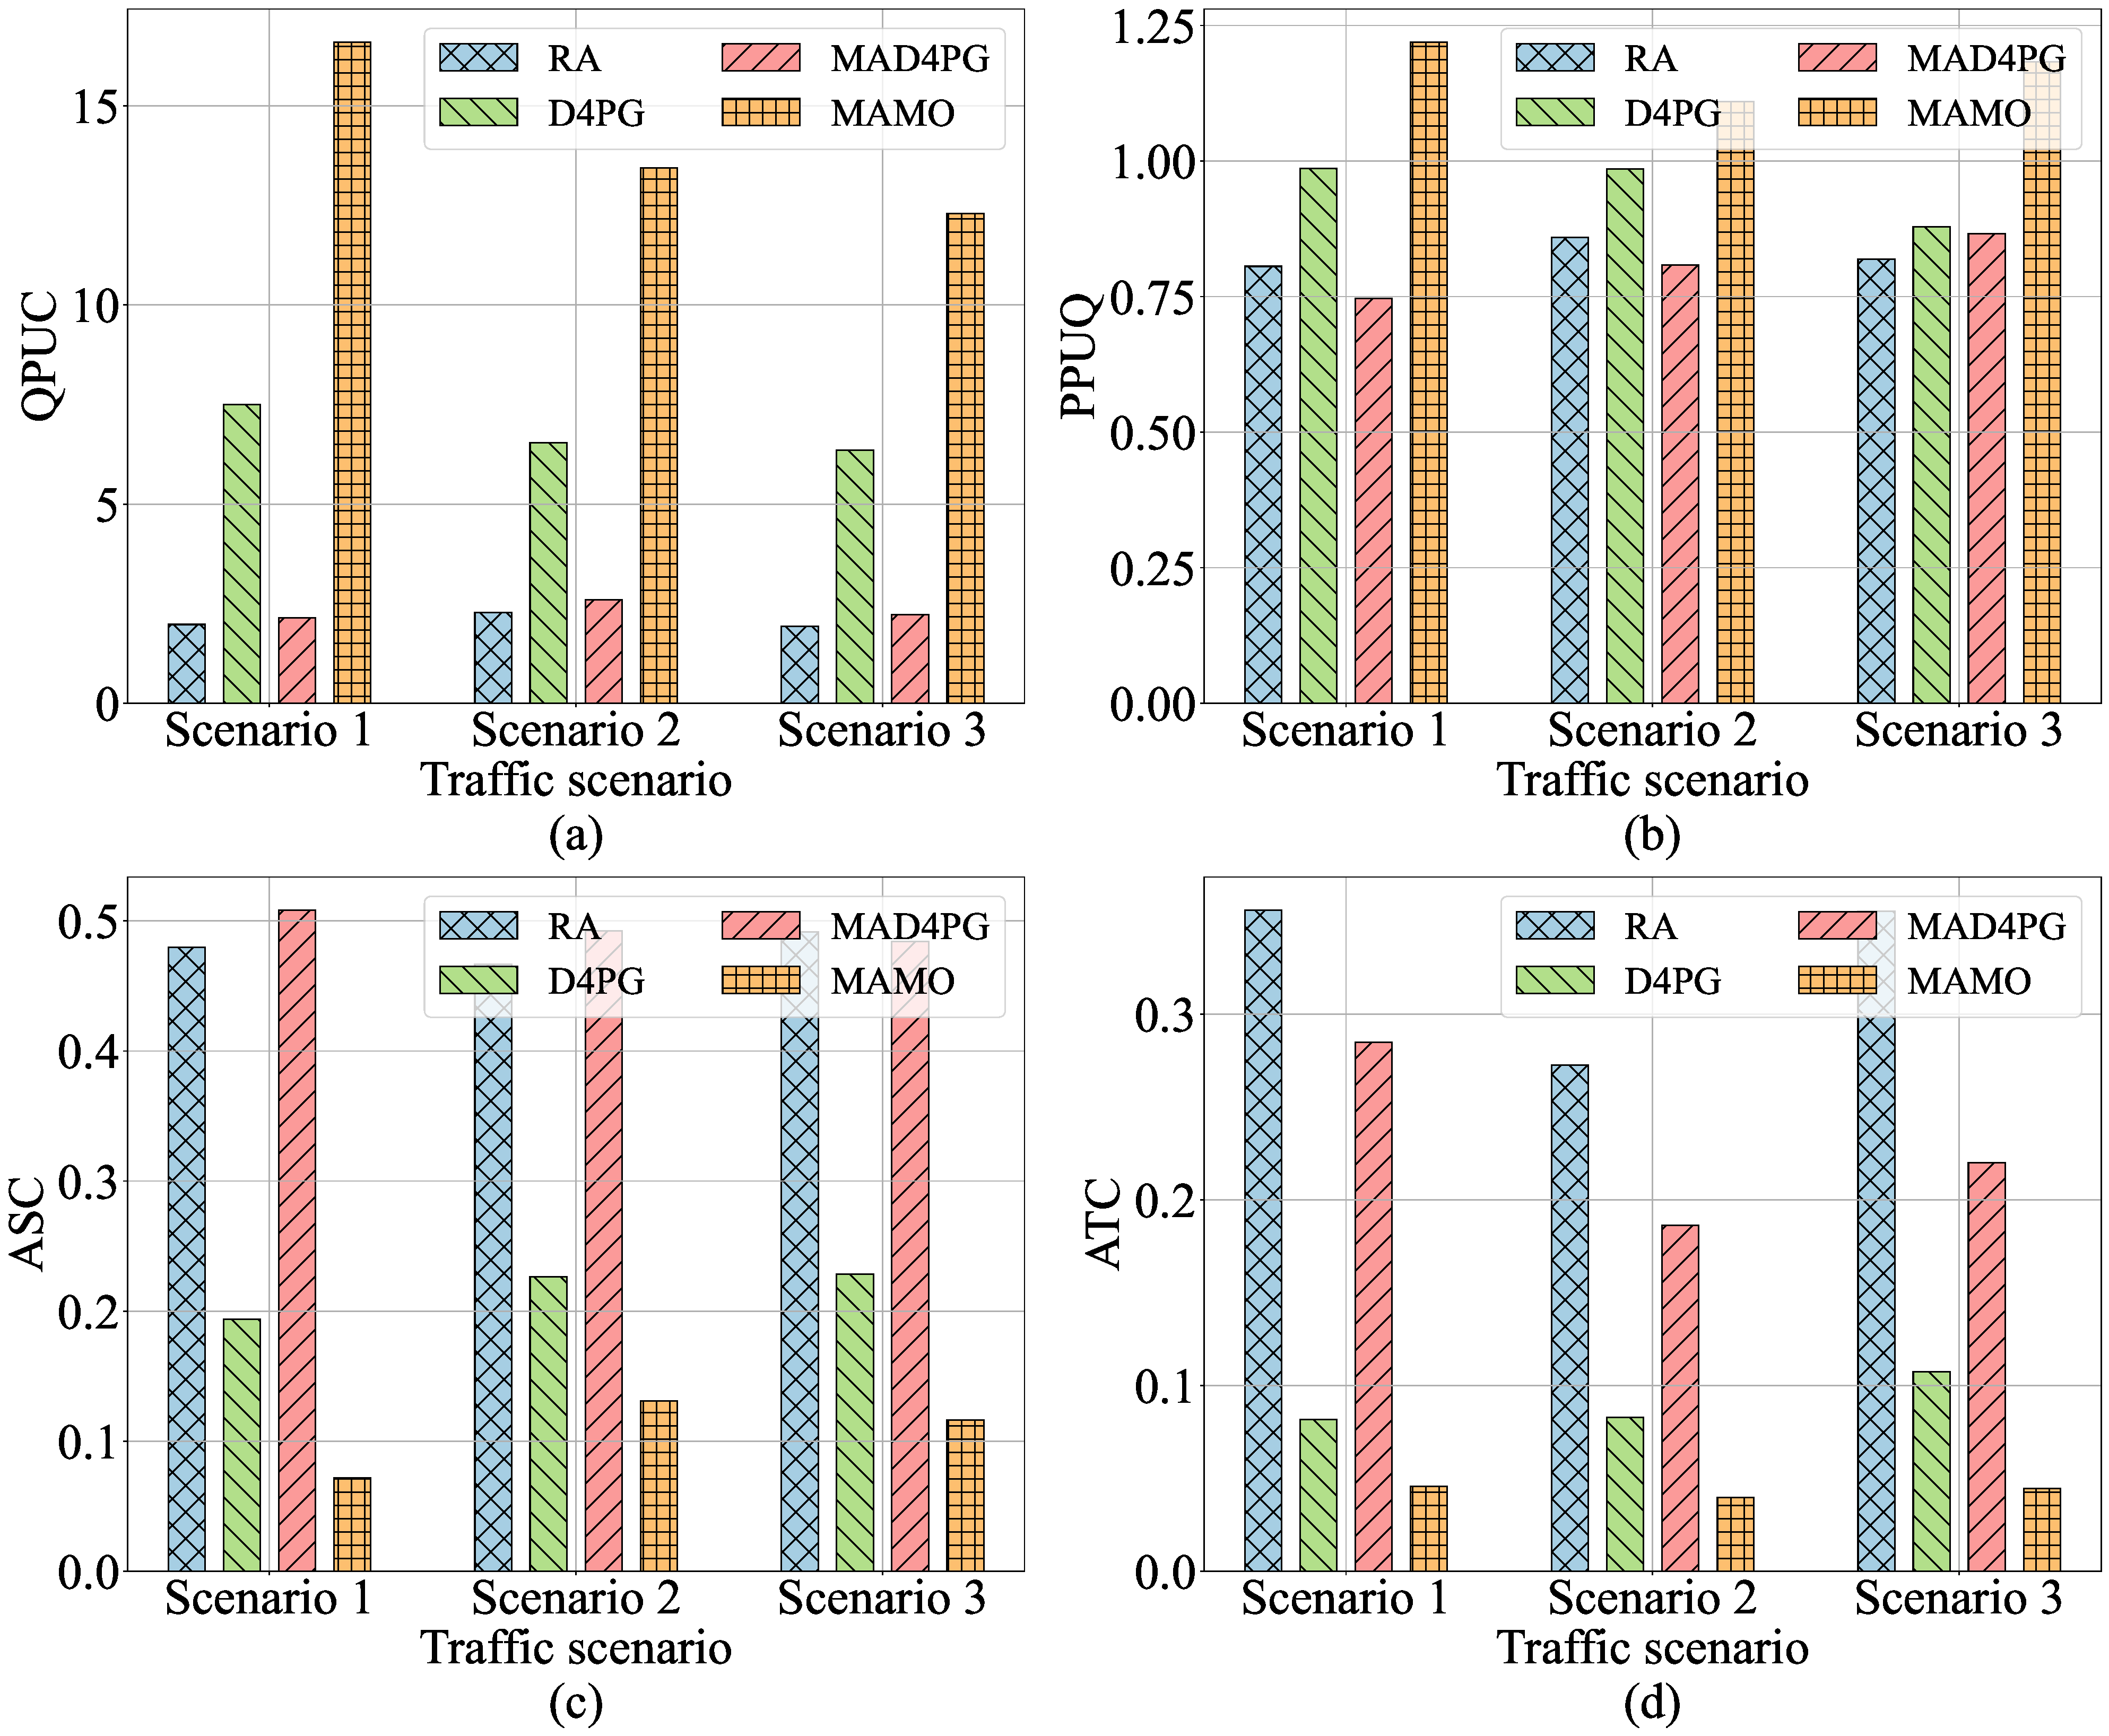
\includegraphics[width=0.55\textwidth]{fig/Fig4-5-different-scenarios.pdf}
	\end{figure}
\end{textblock*}
\end{center}
}

\only<6-6>{

\begin{center} \englishfont \footnotesize
\begin{textblock*}{\textwidth}(-1.75cm,1.6cm)
{\LARGE{\color{red}\ding{216}}}
\end{textblock*}
\end{center}

\begin{center} \englishfont \footnotesize
\begin{textblock*}{\textwidth}(2.2cm,1.6cm)
{\LARGE{\color{red}\ding{216}}}
\end{textblock*}
\end{center}

\begin{center} \englishfont \footnotesize
\begin{textblock*}{\textwidth}(2.2cm,6.85cm)
{\LARGE{\color{red}\ding{216}}}
\end{textblock*}
\end{center}

\begin{center} \englishfont \footnotesize
\begin{textblock*}{\textwidth}(-1.75cm,6.8cm)
{\LARGE{\color{red}\ding{216}}}
\end{textblock*}
\end{center}
}

\only<7-7>{
\frametitle{\englishfont \underline{实验}:V2I带宽的影响}
\begin{center} \englishfont \footnotesize
\begin{textblock*}{\textwidth}(1cm,1.8cm)
	\begin{figure}
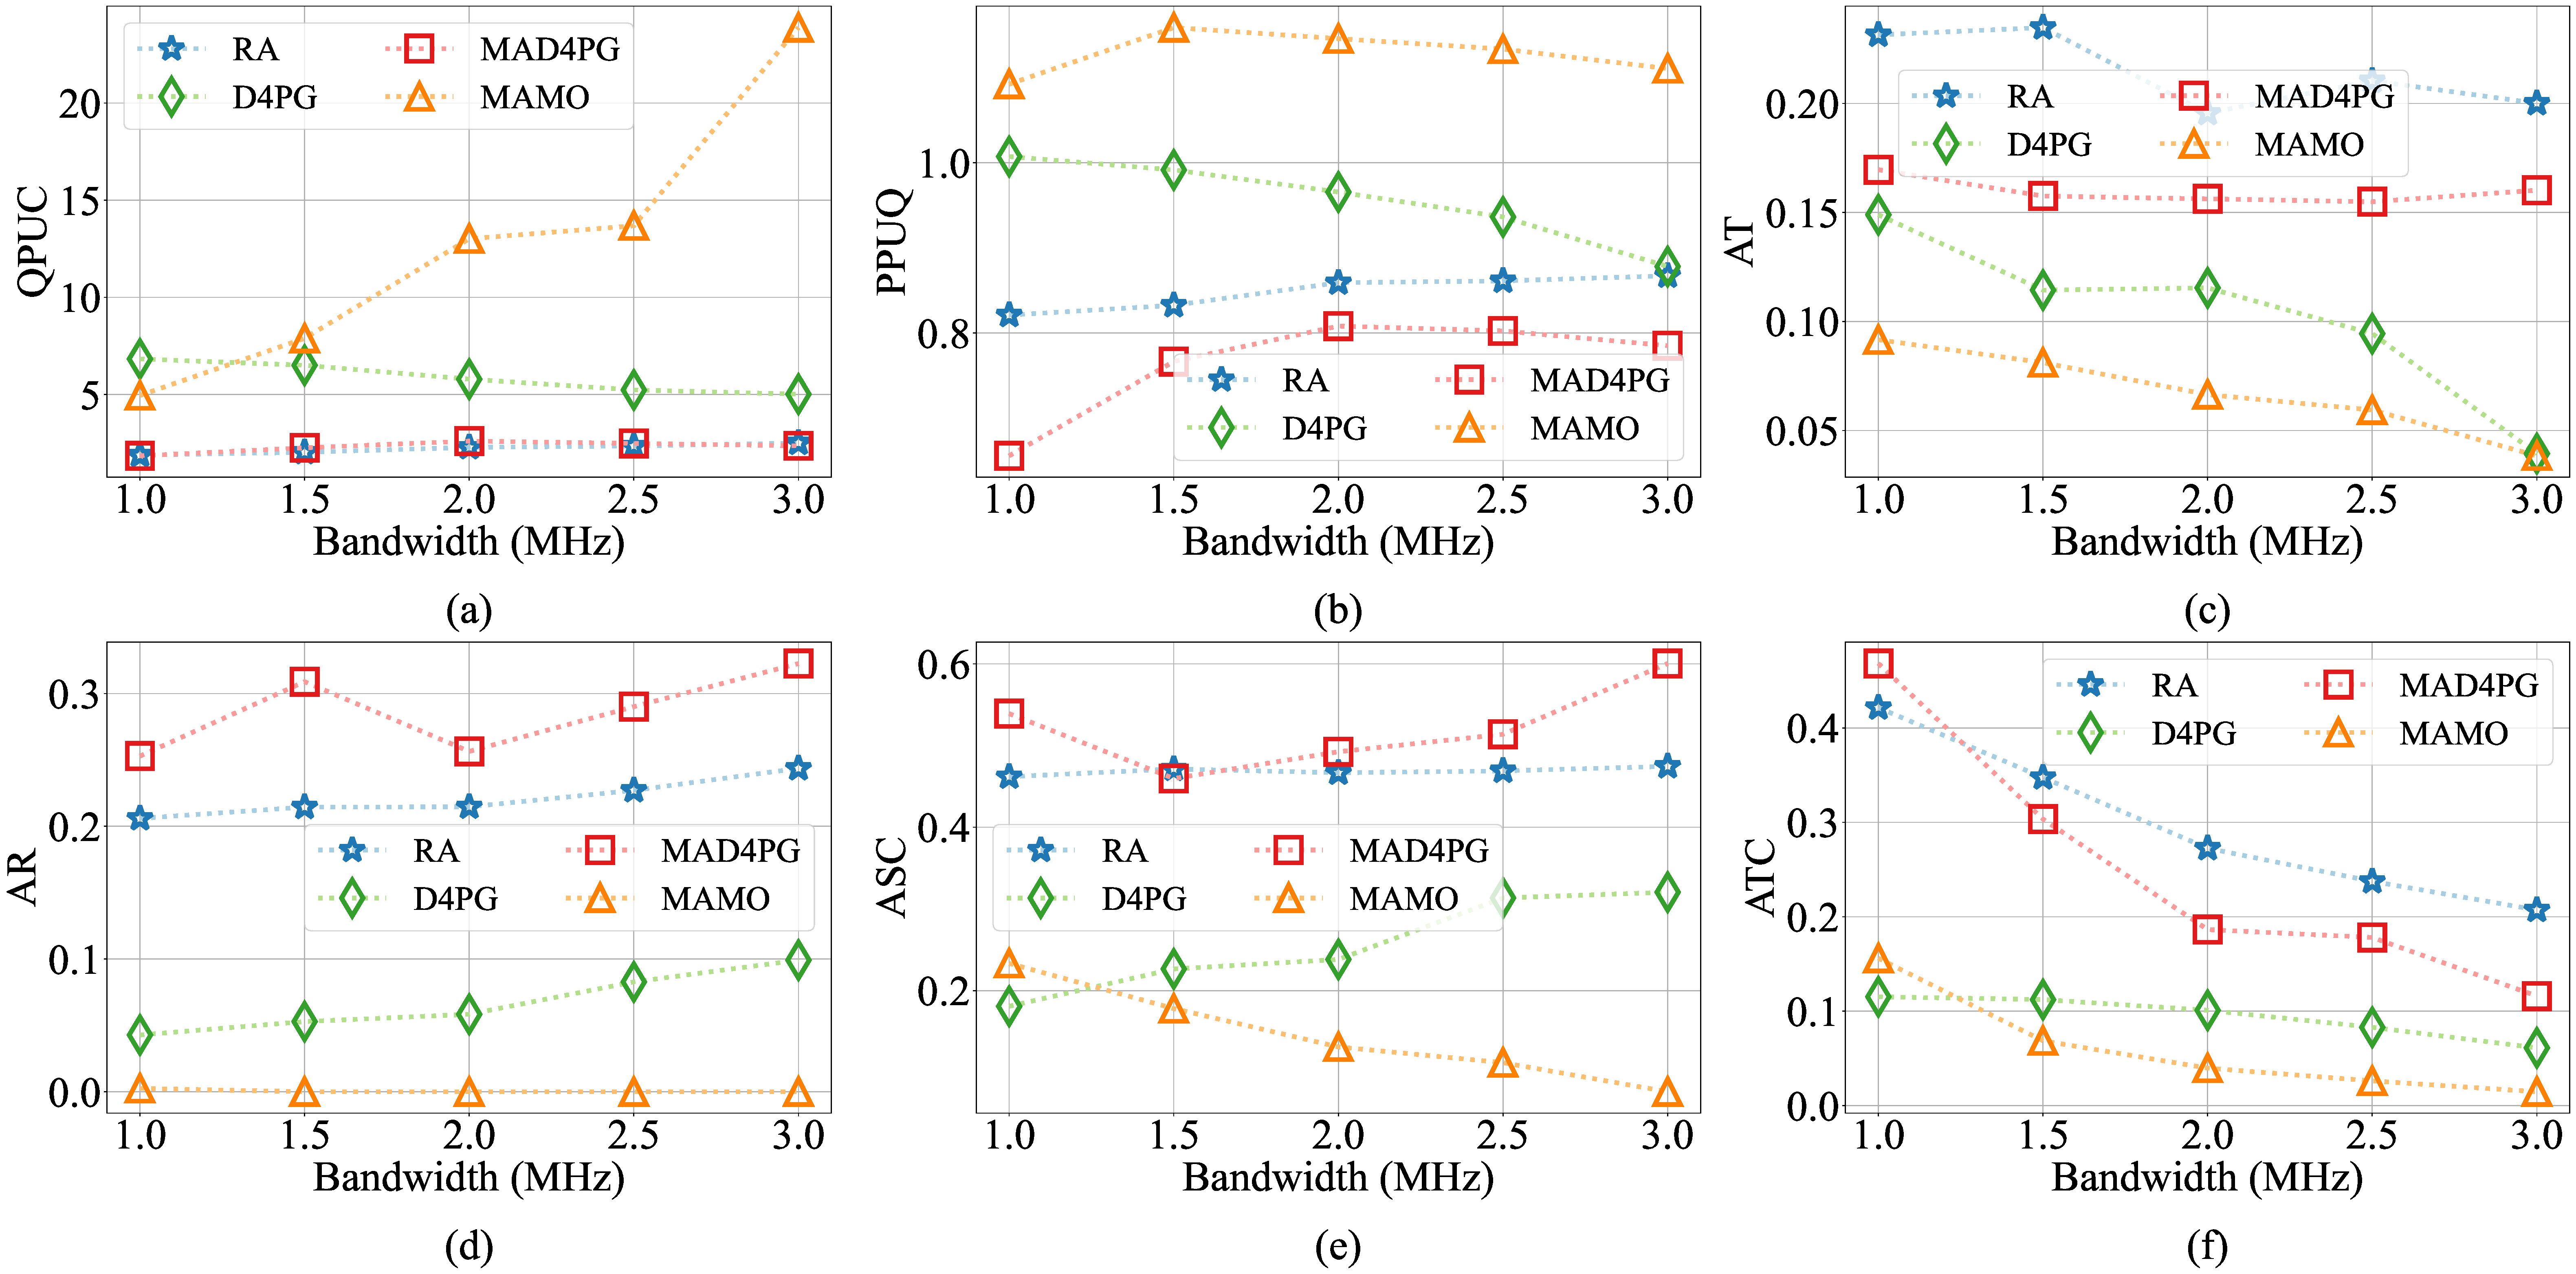
\includegraphics[width=0.9\textwidth]{fig/Fig4-6-different-bandwidths.pdf}
	\end{figure}
\end{textblock*}
\end{center}
}

\only<8-8>{
\frametitle{\englishfont \underline{实验}:V2I带宽的影响}
\begin{center} \englishfont \footnotesize
\begin{textblock*}{\textwidth}(1cm,1.8cm)
	\begin{figure}
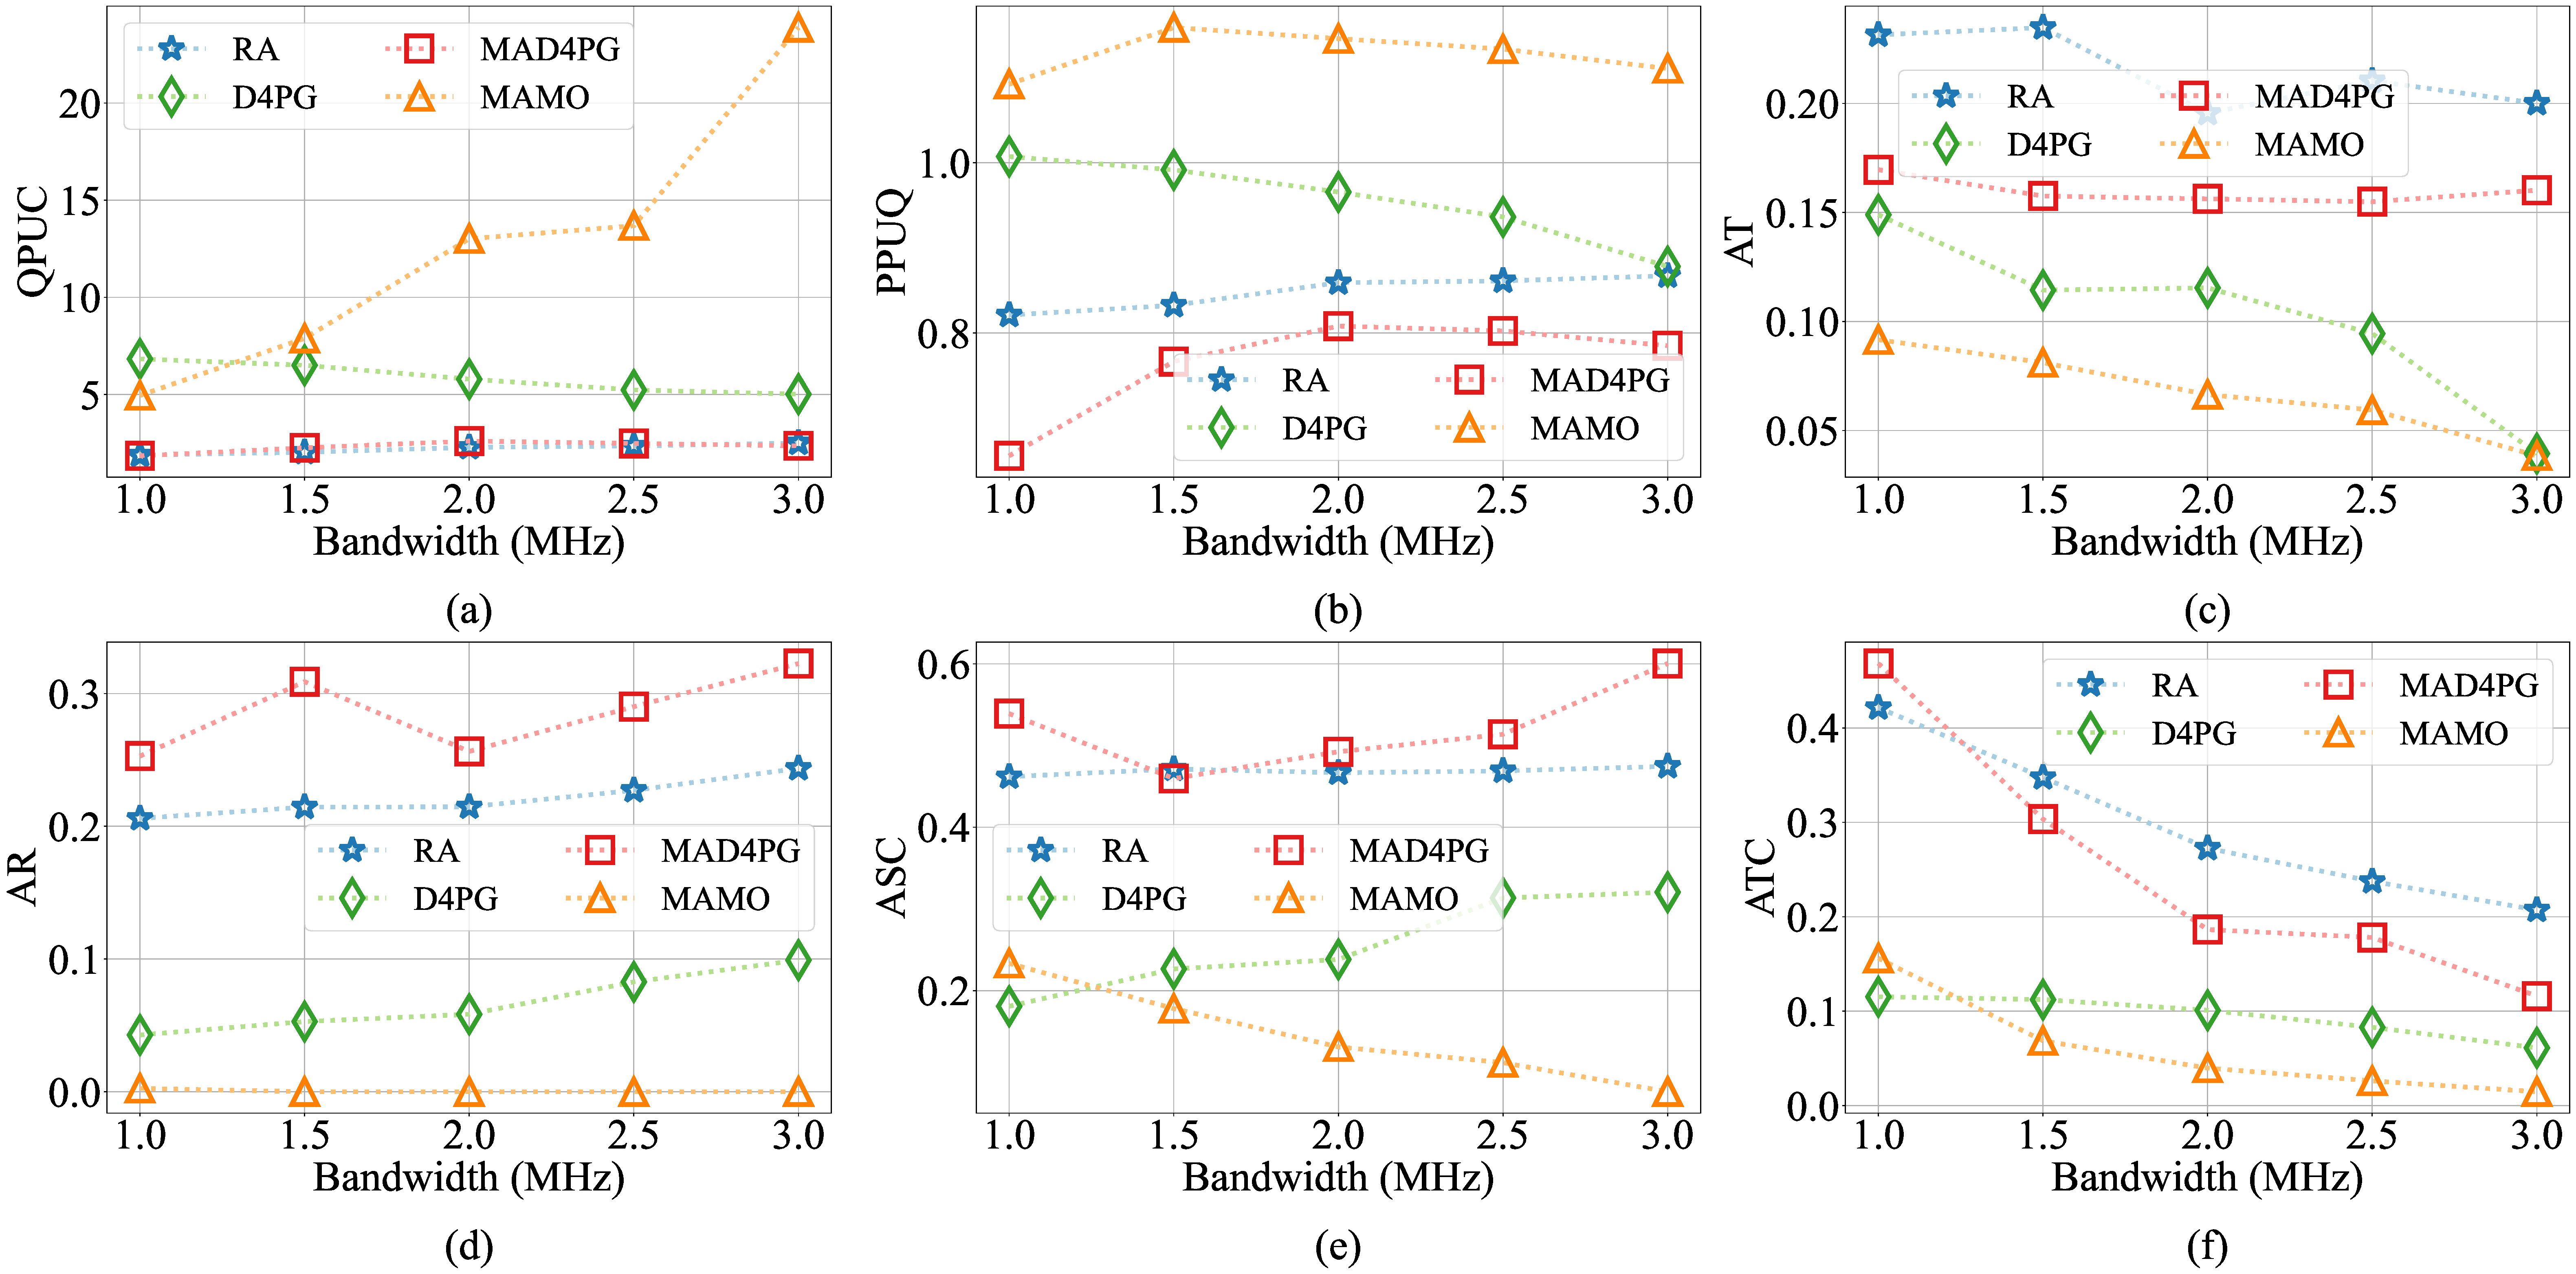
\includegraphics[width=0.9\textwidth]{fig/Fig4-6-different-bandwidths.pdf}
	\end{figure}
\end{textblock*}
\end{center}
}

\only<8-8>{
\begin{center} \englishfont \footnotesize
\begin{textblock*}{\textwidth}(-3.3cm,2.5cm)
{\LARGE{\color{red}\ding{216}}}
\end{textblock*}
\end{center}

\begin{center} \englishfont \footnotesize
\begin{textblock*}{\textwidth}(1cm,1.65cm)
{\LARGE{\color{red}\ding{216}}}
\end{textblock*}
\end{center}

\begin{center} \englishfont \footnotesize
\begin{textblock*}{\textwidth}(5.2cm,3.3cm)
{\LARGE{\color{red}\ding{216}}}
\end{textblock*}
\end{center}

\begin{center} \englishfont \footnotesize
\begin{textblock*}{\textwidth}(-2.7cm,6.8cm)
{\LARGE{\color{red}\ding{216}}}
\end{textblock*}
\end{center}

\begin{center} \englishfont \footnotesize
\begin{textblock*}{\textwidth}(0.65cm,6.46cm)
{\LARGE{\color{red}\ding{216}}}
\end{textblock*}
\end{center}

\begin{center} \englishfont \footnotesize
\begin{textblock*}{\textwidth}(5.65cm,6.65cm)
{\LARGE{\color{red}\ding{216}}}
\end{textblock*}
\end{center}
}

\only<9-9>{
\frametitle{\englishfont \underline{实验}:视图需求的影响}
\begin{center} \englishfont \footnotesize
\begin{textblock*}{\textwidth}(1cm,1.8cm)
	\begin{figure}
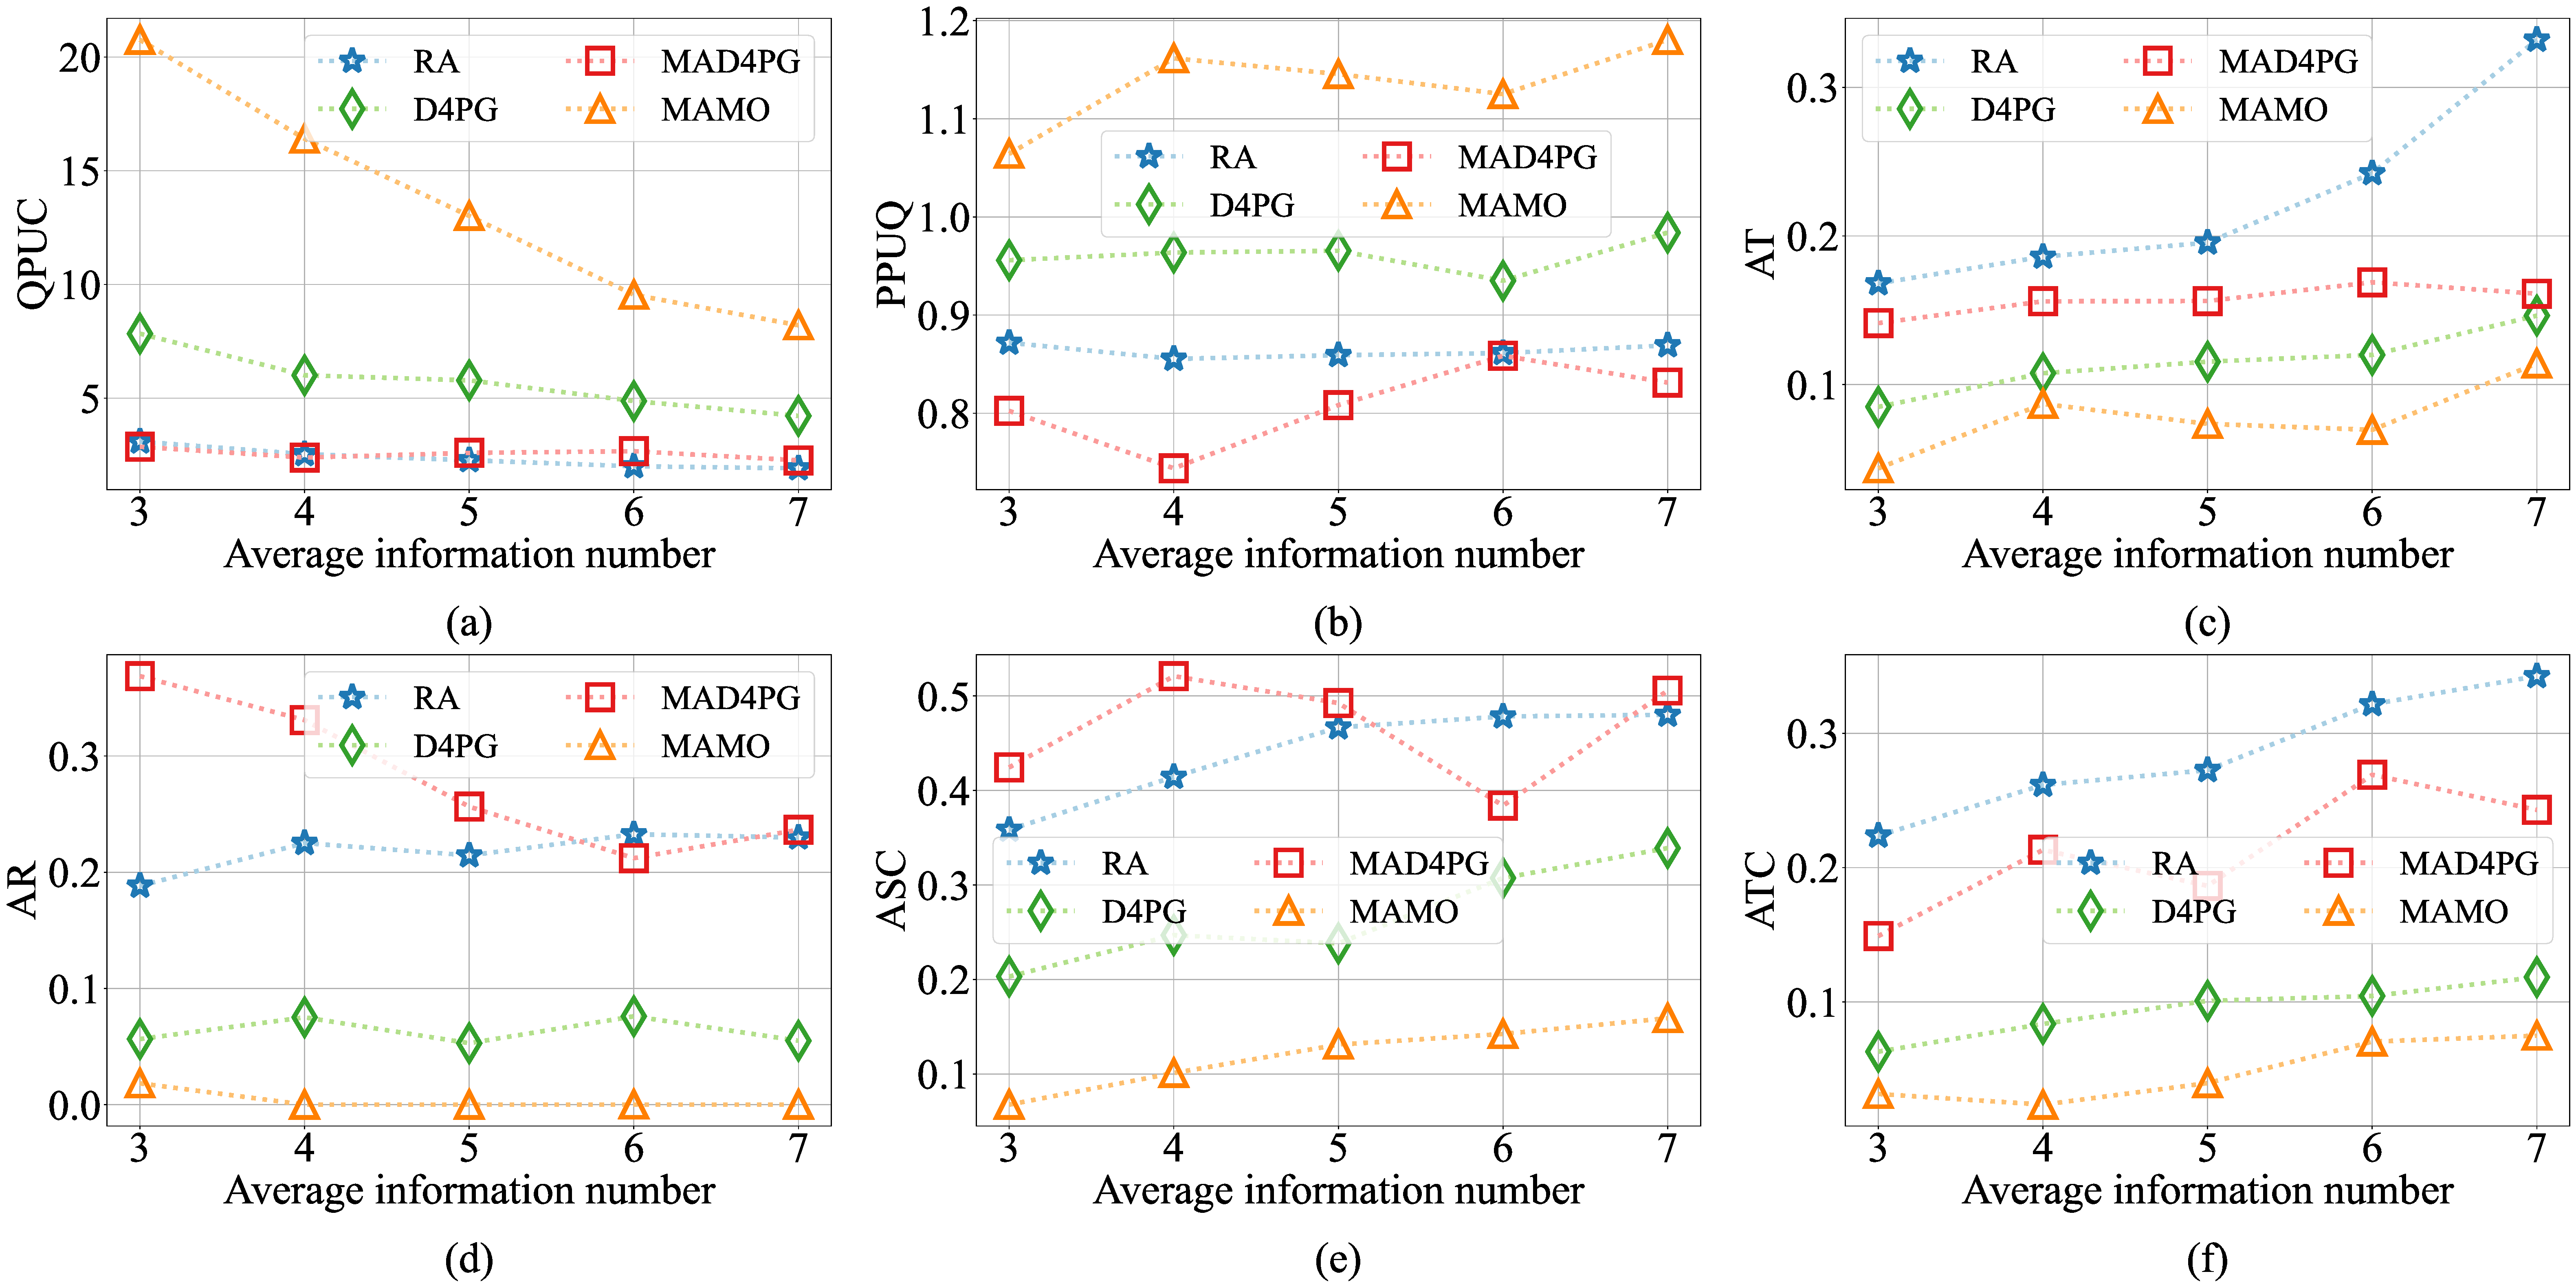
\includegraphics[width=0.9\textwidth]{fig/Fig4-7-different-numbers.pdf}
	\end{figure}
\end{textblock*}
\end{center}
}

\only<10-10>{
\frametitle{\englishfont \underline{实验}:视图需求的影响}
\begin{center} \englishfont \footnotesize
\begin{textblock*}{\textwidth}(1cm,1.8cm)
	\begin{figure}
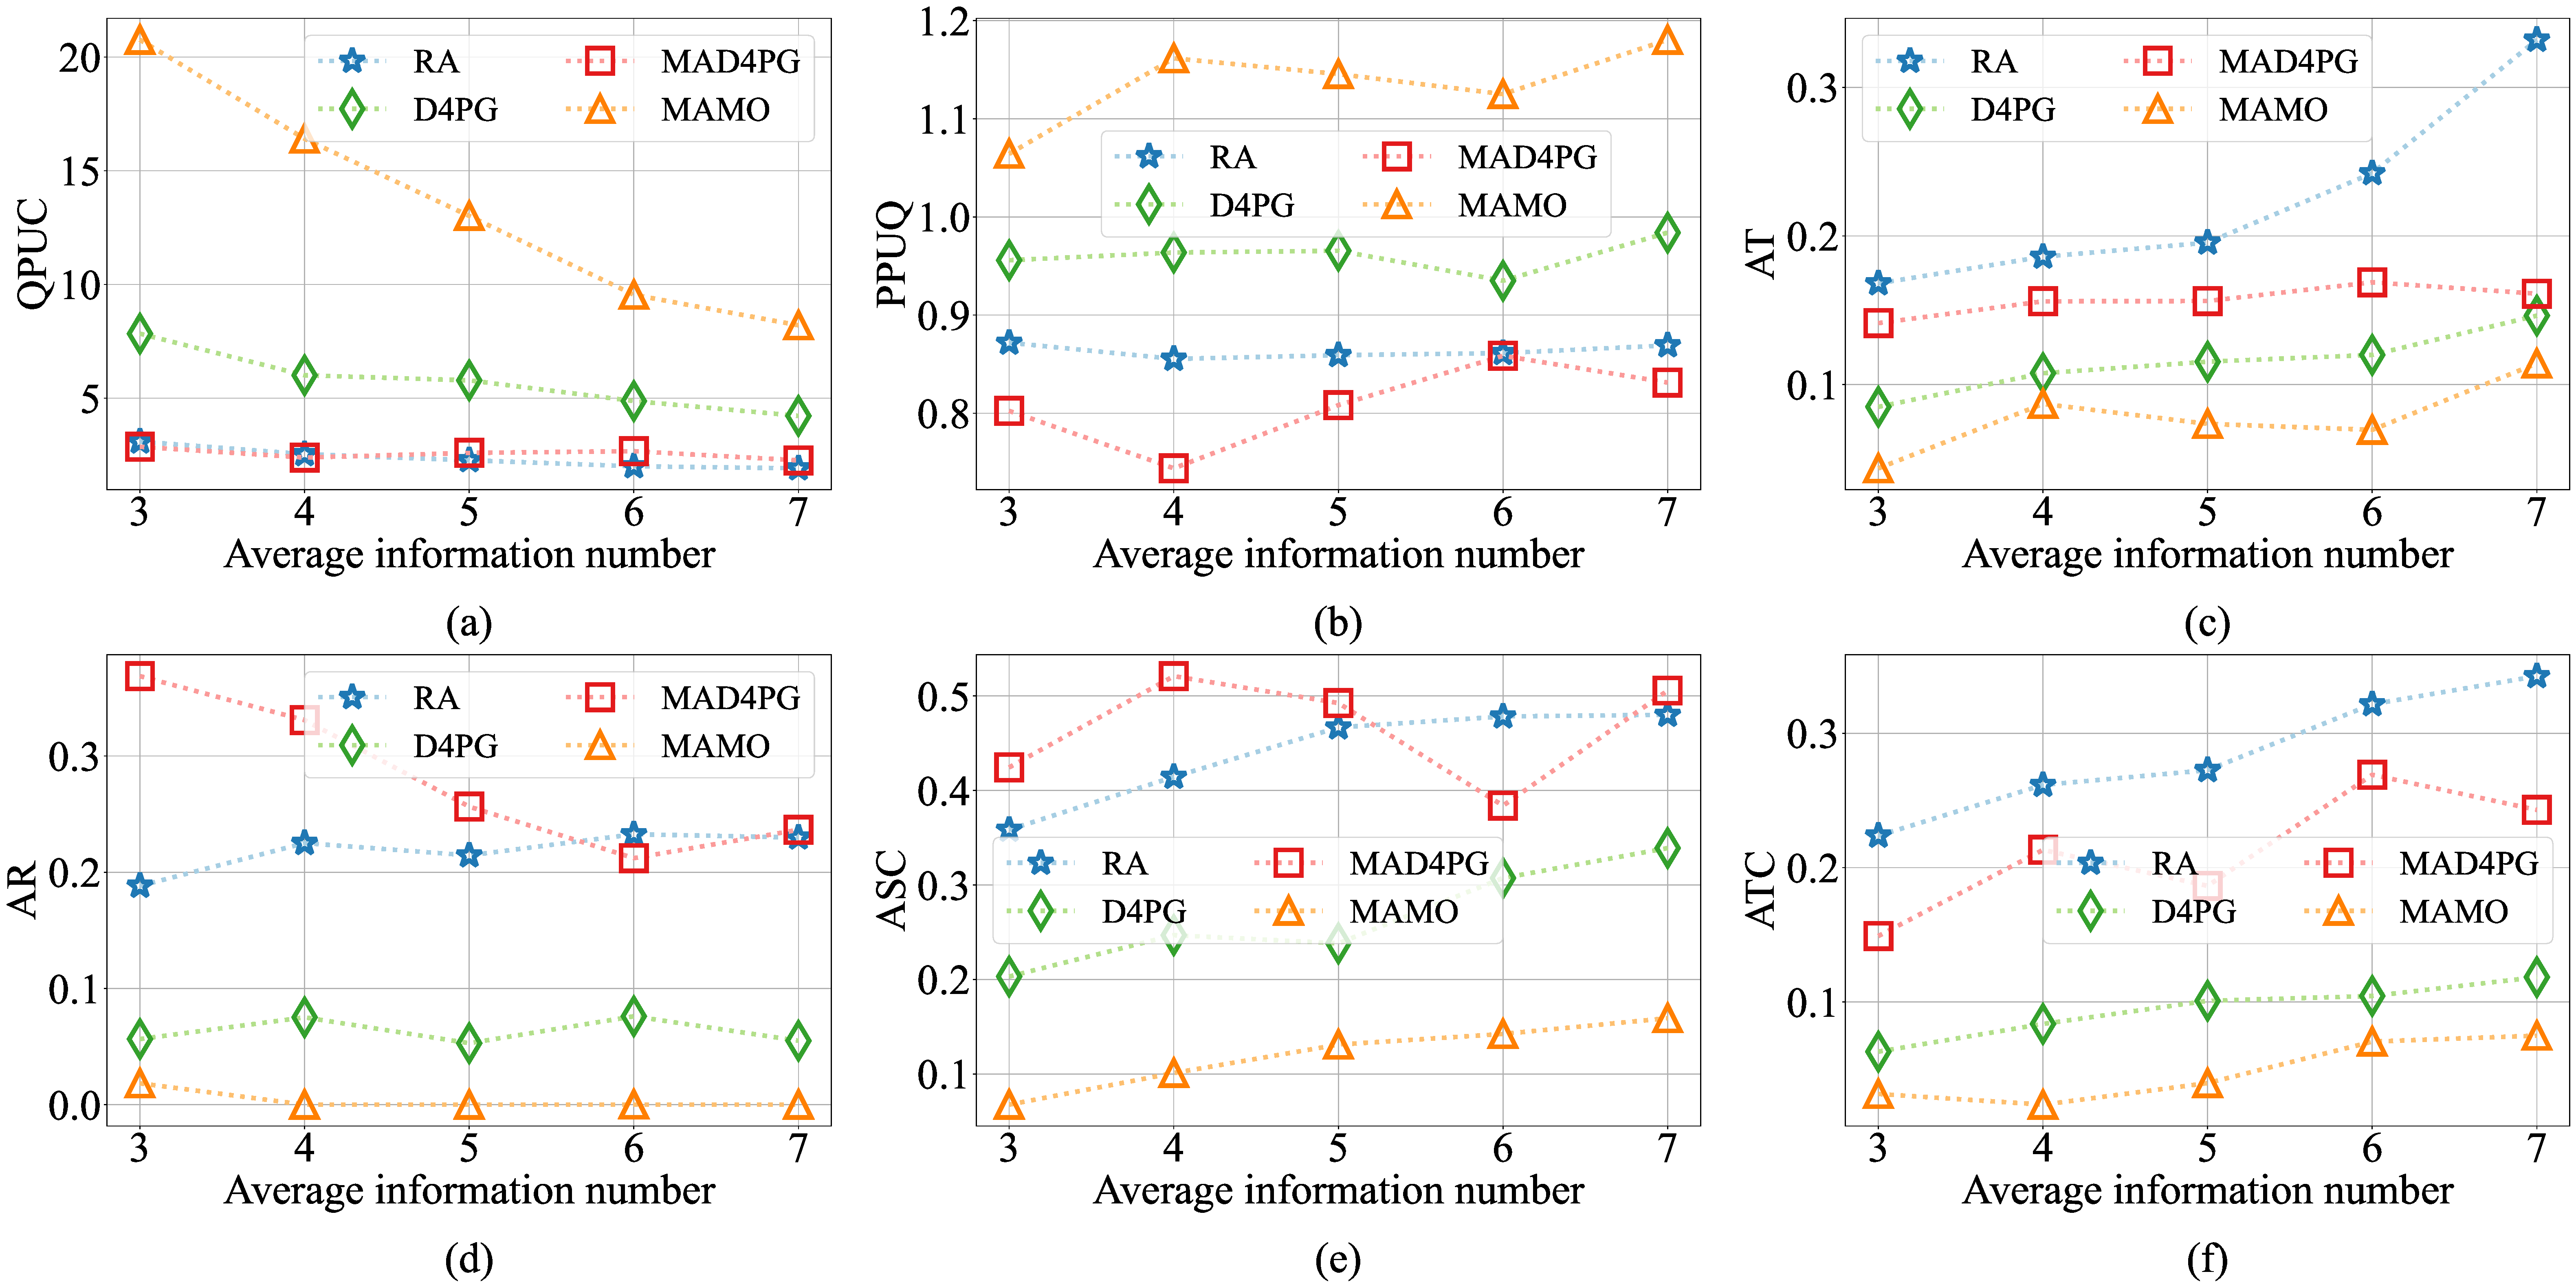
\includegraphics[width=0.9\textwidth]{fig/Fig4-7-different-numbers.pdf}
	\end{figure}
\end{textblock*}
\end{center}
}

\only<10-10>{
\begin{center} \englishfont \footnotesize
\begin{textblock*}{\textwidth}(-4.3cm,1.8cm)
{\LARGE{\color{red}\ding{216}}}
\end{textblock*}
\end{center}

\begin{center} \englishfont \footnotesize
\begin{textblock*}{\textwidth}(0cm,1.75cm)
{\LARGE{\color{red}\ding{216}}}
\end{textblock*}
\end{center}

\begin{center} \englishfont \footnotesize
\begin{textblock*}{\textwidth}(5.2cm,3.45cm)
{\LARGE{\color{red}\ding{216}}}
\end{textblock*}
\end{center}

\begin{center} \englishfont \footnotesize
\begin{textblock*}{\textwidth}(-2.7cm,6.8cm)
{\LARGE{\color{red}\ding{216}}}
\end{textblock*}
\end{center}

\begin{center} \englishfont \footnotesize
\begin{textblock*}{\textwidth}(0.65cm,6.65cm)
{\LARGE{\color{red}\ding{216}}}
\end{textblock*}
\end{center}

\begin{center} \englishfont \footnotesize
\begin{textblock*}{\textwidth}(5.65cm,6.65cm)
{\LARGE{\color{red}\ding{216}}}
\end{textblock*}
\end{center}
}
\end{overlayarea}
\end{frame}
